\def\filepath{templates}
%\def\filepath{C:/Users/holden-lee/Dropbox/Math/templates}

\documentclass[12pt]{book}
\usepackage{etex}
%this prevents the "No room for a new \dimen" error that comes from loading too many packages (tikz+xy in particular)

%load geometry first (sets up page)
\usepackage[top=1.2in, bottom=1.2in, left=1in, right=1in]{geometry}

%main packages
\usepackage{amscd}
\usepackage{amsmath}
\usepackage{amssymb}
\usepackage{amsthm}
\usepackage{array}
\usepackage{bbm}
%\usepackage{asymptote}
\usepackage{cancel}
\usepackage{chemarrow}
\usepackage{cmap}
\usepackage{courier}
\usepackage[usenames,dvipsnames]{color}%%%
%\usepackage{color}
%\usepackage{ctable}
\usepackage{enumerate}
\usepackage{enumitem}%resume lists
\usepackage{fancyhdr}
\usepackage{listings}
\lstset{
	basicstyle=\small\ttfamily,
	keywordstyle=\color{blue},
	language=python,
	xleftmargin=16pt,
}
\usepackage{makeidx}
%\usepackage{marvosym}%doesn't work
\usepackage{mathdots}%iddots: dots going northeast
\usepackage{mathtools}
\usepackage{mathrsfs}
%\usepackage{hyperref}
%\usepackage{sidecap}
\usepackage{stackrel}
\usepackage{stmaryrd}%\mapsfrom
\usepackage{tabularx}
\usepackage{tikz}
\usepackage{titlesec}
\usepackage{titletoc}
\usepackage{url}
\usepackage{verbatim}
\usepackage{wasysym}
\usepackage{wrapfig}
\usepackage{yhmath}
%\usepackage{yhmath}%arcs
\usepackage[all,cmtip]{xy}%Commutative diagrams
%\usepackage[usenames,dvipsnames]{xcolor}%tikz loads xcolor


\usepackage[usenames,dvipsnames]{color} % Required for specifying custom colors and referring to colors by name
\usepackage[pdftex]{hyperref} % For hyperlinks in the PDF
\hypersetup{
  colorlinks=true,
  linkcolor=MyBlue, 
  citecolor=MyRed,
  urlcolor= MyBlue
}

\definecolor{MyRed}{rgb}{0.99, 0.0, 0.0} 
\definecolor{MyGreen}{rgb}{0.0,0.4,0.0} 
\definecolor{MyBlue}{rgb}{0.0, 0.0, 0.6}

%load hyperref last
%\usepackage{hyperref}
%\usepackage{listings}
%\lstset{
%	basicstyle=\small\ttfamily,
%	keywordstyle=\color{blue},
%	language=python,
%	xleftmargin=16pt,
%}
%this causes an error. No idea why.

\usetikzlibrary{calc,trees,positioning,arrows,chains,shapes.geometric,%
    decorations.pathreplacing,decorations.pathmorphing,shapes,%
    matrix,shapes.symbols,shadows,fadings}

%\input xy
%\xyoption{all}

%http://www.simonsilk.com/content/simonsilk/2011-jun/latex-list-notations-nomenclature
\usepackage[refpage]{nomencl}
\renewcommand{\nomname}{List of Notations}
\renewcommand*{\pagedeclaration}[1]{\unskip\dotfill\hyperpage{#1}}
\makenomenclature
%The first line invokes the nomenclature package, and the option refpage means that the list will include, for each symbol in the list,  the page number on which you added it with the \nomenclature command. Leave it out to remove page numbers. The second line is the title at the top of the list of notations. The third line changes the page numbers in the list so they are right-justified with a line of dots connecting them back to the description of the symbol. By default, they follow the description after a comma and the word "page." The last line tells Latex you're using nomenclature so it will generate and look for the associated intermediate files during successive runs.

\makeindex

\setcounter{tocdepth}{3}
\setcounter{secnumdepth}{3}
%\pagenumbering{arabic}

%http://tex.stackexchange.com/questions/142982/how-to-get-the-current-chapter-name-section-name-subsection-name-etc?lq=1
\usepackage{etoolbox}
% Patch the sectioning commands to provide a hook to be used later
\preto{\chapter}{\def\leveltitle{\chaptertitle}}
\preto{\section}{\def\leveltitle{\sectiontitle}}
\preto{\subsection}{\def\leveltitle{\subsectiontitle}}
\preto{\subsubsection}{\def\leveltitle{\subsubsectiontitle}}

\makeatletter
% \@sect is called with normal sectioning commands
% Argument #8 to \@sect is the title
% Thus \section{Title} will do \gdef\sectiontitle{Title}
\pretocmd{\@sect}
  {\expandafter\gdef\leveltitle{#8}}
  {}{}
% \@ssect is called with *-sectioning commands
% Argument #5 to \@ssect is the title
\pretocmd{\@ssect}
  {\expandafter\gdef\leveltitle{#5}}
  {}{}
% \@chapter is called by \chapter (without *)
% Argument #2 to \@chapter is the title
\pretocmd{\@chapter}
  {\expandafter\gdef\leveltitle{#2}}
  {}{}
% \@schapter is called with \chapter*
% Argument #1 to \@schapter is the title
\pretocmd{\@schapter}
  {\expandafter\gdef\leveltitle{#1}}
  {}{}
\makeatother
%%%%%%%%%%%%%%%%%%%%%%%%%%%%%%%%%%%%%%%%%%%%%%%%%
%%%Theorem styles
\newtheoremstyle{norm}
{12pt}
{12pt}
{}
{}
{\bf}
{:}
{.5em}
{}

\newtheorem{thm}{Theorem}[section]
\newtheorem*{thm*}{Theorem}
\newtheorem{clm}[thm]{Claim}
\newtheorem*{clm*}{Claim}
\newtheorem{conj}[thm]{Conjecture}
\newtheorem*{conj*}{Conjecture}
%\newtheorem{cons}{Construction}
\newtheorem{cor}[thm]{Corollary}
\newtheorem{lem}[thm]{Lemma}
\newtheorem*{lem*}{Lemma}

\theoremstyle{norm}
\newtheorem{prb}[thm]{Problem}%[section]
\newtheorem*{prb*}{Problem}

\newtheorem{alg}[thm]{Algorithm}
\newtheorem{ax}[thm]{Axiom}
\newtheorem*{ax*}{Axiom}
\newtheorem{df}[thm]{Definition}
\newtheorem*{df*}{Definition}
\newtheorem{ex}[thm]{Example}
\newtheorem*{ex*}{Example}
\newtheorem{exr}[thm]{Exercise}
\newtheorem{expl}[thm]{Exploration}%prb
\newtheorem{fct}[thm]{Fact}
\newtheorem{mdl}[thm]{Model}
\newtheorem{pos}[thm]{Postulate}
\newtheorem*{pos*}{Postulate}
%\newtheorem{sprb}{Problem}%numbering for solutions
\newtheorem{pr}[thm]{Proposition}
\newtheorem*{pr*}{Proposition}
\newtheorem{qu}[thm]{Question}
\newtheorem*{qu*}{Question}
\newtheorem{rem}[thm]{Remark}
\newtheorem*{rem*}{Remark}

%%%%%%%%%%%%%%%%%%%%%%%%%%%%%%%%%%%%%%%%%%%%%%%%%

%%%%%%%%%%%%%%%%%%%%%%%%%%%%%%%%%%%%%%%%%%%%%%%%%
%%DEFINING BOX COMMANDS
\newcommand{\prbox}[1]{{
\noindent
\centering
\begin{tikzpicture}
\node [prbox] (box){
\begin{minipage}[l]{6in}
#1
\end{minipage}
};
\end{tikzpicture}\\%
}
}
\newcommand{\prbbox}[1]{\prbox{\begin{prb}#1\end{prb}}}
\newcommand{\expbox}[1]{\prbox{\begin{expl}#1\end{expl}}}
\newcommand{\sprbbox}[1]{\prbox{\begin{sprb}#1\end{sprb}}}

\newcommand{\thbox}[1]{{
\noindent
\centering
\begin{tikzpicture}
\node [thbox] (box){
\begin{minipage}[l]{6in}
#1
\end{minipage}
};
\end{tikzpicture}\\%
}}
%6.68

\newcommand{\thmbox}[1]{\thbox{\begin{thm}#1\end{thm}}}
\newcommand{\dfbox}[1]{\thbox{\begin{df*}#1\end{df*}}}

\newcommand{\grbox}[1]{{
\noindent
\centering
\begin{tikzpicture}
\node [cpbox] (box){
\begin{minipage}[l]{6in}
#1
\end{minipage}
};
\end{tikzpicture}\\%
}}
\newcommand{\cpbox}[1]{{
\noindent
\centering
\begin{tikzpicture}
\node [cpbox] (box){
\begin{minipage}[c]{.2in}
%\hspace{-.2in}
%\dbend
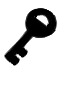
\includegraphics[scale=0.35]{\filepath/key}
\end{minipage}
\begin{minipage}[t]{6in}%6.25
#1
\end{minipage}
};
\end{tikzpicture}\\%
}}


\newcommand{\wrbox}[1]{{
\noindent
\centering
\begin{tikzpicture}
\node [wrbox] (box){
\begin{minipage}[c]{.2in}
%\hspace{-.2in}
%\dbend
{\Huge \bf !}
\end{minipage}
\begin{minipage}[t]{6in}%6.25
#1
\end{minipage}
};
\end{tikzpicture}\\%
}}
\newcommand{\hintbox}[1]{{
\noindent
\centering
\begin{tikzpicture}
\node [hnbox] (box){
\begin{minipage}[l]{6in}
\textbf{Hint:} {#1}
\end{minipage}
};
\end{tikzpicture}\\%
}
}
%white box
\newcommand{\whbox}[1]{{
\noindent
\centering
\begin{tikzpicture}
\node [hnbox] (box){
\begin{minipage}[l]{6in}
{#1}
\end{minipage}
};
\end{tikzpicture}\\%
}
}
%6.68
%END DEFINING BOX COMMANDS
%%%%%%%%%%%%%%%%%%%%%%%%%%%%%%%%%%%%%%%%%%%%%%%%%

%Box commands
%\thbox{...} makes a theorem box
%\thmbox{...} makes a theorem box labeled "Theorem"
%\prbox{...} makes a problem box
%\prbbox{...} makes a problem box labeled "Problem"
%\cpbox{...} makes a concept box labeled "Concept"
%\wrbox{...} makes a warning box.
%\dfbox{...} makes a definition box (same as problem box) labeled "> Definition"
%\sprbbox{...} makes a problem box labeled "Problem" (use this when you're making a copy of a previous problem box to put the solution afterwards; it has a numbering system separate from problems).

 
% for testing purposes only
\usepackage[english]{babel} 
\usepackage{blindtext} 
%%%%%%%%
%begin doc
%%%%%%%%
%%%%%%%%%%%%%%%%%%%%%%%%%%%%%%%%%%%%%%%%%%%%%%%%%
%DEFINING THE BOXES.
% Problem box (simple box, blue)
\tikzstyle{prbox} = [draw=black, fill=blue!20, very thick,
    rectangle, inner sep=10pt, inner ysep=10pt]
% Theorem box (double border, gray)
\tikzstyle{thbox} = [draw=black,double, fill=blue!10, very thick,
    rectangle, inner sep=10pt, inner ysep=10pt]
%\tikzstyle{fancytitle} =[fill=red, text=white]
% Concept box (shadowed, light green)
\tikzstyle{cpbox} = [drop shadow={
    shadow scale=1}, draw=black, fill=green!10, very thick,
    rectangle, inner sep=10pt, inner ysep=10pt]
\tikzstyle{wrbox} = [drop shadow={
    shadow scale=1}, draw=black, fill=yellow!10, very thick,
    rectangle, inner sep=10pt, inner ysep=10pt]
\tikzstyle{hnbox} = [draw=black, fill=white, very thick,
    rectangle, inner sep=10pt, inner ysep=10pt]
%END DEFINING BOXES
%%%%%%%%%%%%%%%%%%%%%%%%%%%%%%%%%%%%%%%%%%%%%%%%%

%LETTERS

%UPPERCASE
\newcommand{\sA}[0]{\mathscr{A}}
\newcommand{\cA}[0]{\mathcal{A}}
\newcommand{\A}[0]{\mathbb{A}}
\newcommand{\cB}[0]{\mathcal{B}}
\newcommand{\C}[0]{\mathbb{C}}
\newcommand{\sC}[0]{\mathcal{C}}%deprecated
\newcommand{\cC}[0]{\mathcal{C}}
\newcommand{\sD}[0]{\mathscr{D}}
\newcommand{\mD}[0]{\mathfrak D}
\newcommand{\cE}[0]{\mathscr{E}}%deprecated
\newcommand{\sE}[0]{\mathscr{E}}
\newcommand{\E}[0]{\mathbb{E}}
\newcommand{\EE}[0]{\mathop{\mathbb E}}
%\scalebox{1.25}{$\mathbb E$}}
\newcommand{\F}[0]{\mathbb{F}}
\newcommand{\cF}[0]{\mathcal{F}}
\newcommand{\sF}[0]{\mathscr{F}}
\newcommand{\G}[0]{\mathbb{G}}
\newcommand{\cG}[0]{\mathscr{G}}%deprecated.
\newcommand{\sG}[0]{\mathscr{G}}
\newcommand{\cH}[0]{\mathscr H}%deprecated
\newcommand{\sH}[0]{\mathscr H}
\newcommand{\Hq}[0]{\mathbb{H}}
\newcommand{\bfI}[0]{\mathbf{I}}
\newcommand{\I}[0]{\mathbb{I}}
\newcommand{\cI}[0]{\mathscr{I}}%deprecated
\newcommand{\sI}[0]{\mathscr{I}}
\newcommand{\cJ}[0]{\mathscr{J}}
\newcommand{\cL}[0]{\mathscr{L}}
\newcommand{\mM}[0]{\mathfrak{M}}
\newcommand{\N}[0]{\mathbb{N}}
\newcommand{\fN}[0]{\mathfrak{N}}
\newcommand{\cP}[0]{\mathcal{P}}
\newcommand{\Pj}[0]{\mathbb{P}}
\newcommand{\mP}[0]{\mathfrak{P}}
\newcommand{\mQ}[0]{\mathfrak{Q}}
%!
\newcommand{\cO}[0]{\mathcal{O}}
\newcommand{\sO}[0]{\mathscr{O}}
\newcommand{\Q}[0]{\mathbb{Q}}
\newcommand{\R}[0]{\mathbb{R}}
\newcommand{\bS}[0]{\mathbb{S}}
\newcommand{\T}[0]{\mathbb{T}}
\newcommand{\X}[0]{\mathfrak{X}}
\newcommand{\Z}[0]{\mathbb{Z}}
\newcommand{\one}[0]{\mathbbm{1}}
%lowercase
\newcommand{\mba}[0]{\mathbf{a}}%idele a
\newcommand{\ma}[0]{\mathfrak{a}}%ideal a
\newcommand{\mb}[0]{\mathfrak{b}}
\newcommand{\mc}[0]{\mathfrak{c}}
\newcommand{\mfd}[0]{\mathfrak d}
\newcommand{\mf}[0]{\mathfrak{f}}
\newcommand{\fg}[0]{\mathfrak{g}}
\newcommand{\vi}[0]{\mathbf{i}}%vector i
\newcommand{\vj}[0]{\mathbf{j}}
\newcommand{\vk}[0]{\mathbf{k}}
\newcommand{\mm}[0]{\mathfrak{m}}%ideal m
\newcommand{\mfp}[0]{\mathfrak{p}}
\newcommand{\mq}[0]{\mathfrak{q}}
\newcommand{\mr}[0]{\mathfrak{r}}
\newcommand{\mv}[0]{\mathbf{v}}
\newcommand{\mx}[0]{\mathbf{x}}%idele x
\newcommand{\my}[0]{\mathbf{y}}
%More sequences of letters
\newcommand{\et}[0]{_{\text{\'et}}}
\newcommand{\Gm}[0]{\mathbb{G}_m}
\newcommand{\Fp}[0]{\mathbb{F}_p}
\newcommand{\fq}[0]{\mathbb{F}_q}
\newcommand{\fpb}[0]{\ol{\mathbb{F}_p}}
\newcommand{\fpt}[0]{\mathbb{F}_p^{\times}}
\newcommand{\fqt}[0]{\mathbb{F}_q^{\times}}
\newcommand{\Kt}[0]{K^{\times}}
\newcommand{\RP}[0]{\mathbb{R}P}
\newcommand{\qb}[0]{\ol{\mathbb{Q}}}
\newcommand{\qp}[0]{\mathbb{Q}_p}
\newcommand{\qpb}[0]{\ol{\mathbb{Q}_p}}
\newcommand{\ql}[0]{\mathbb Q_{\ell}}
\newcommand{\sll}[0]{\mathfrak{sl}}
\newcommand{\vl}[0]{V_{\ell}}
\newcommand{\zl}[0]{\mathbb Z_{\ell}}
\newcommand{\zp}[0]{\mathbb Z_{p}}
\newcommand{\zpz}[0]{\mathbb Z/p\mathbb Z}
%Shortcuts for greek letters
\newcommand{\al}[0]{\alpha}
\newcommand{\be}[0]{\beta}
\newcommand{\ga}[0]{\gamma}
\newcommand{\Ga}[0]{\Gamma}
\newcommand{\de}[0]{\delta}
\newcommand{\De}[0]{\Delta}
\newcommand{\ep}[0]{\varepsilon}
\newcommand{\eph}[0]{\frac{\varepsilon}{2}}
\newcommand{\ept}[0]{\frac{\varepsilon}{3}}
\newcommand{\ka}[0]{\kappa}
\newcommand{\la}[0]{\lambda}
\newcommand{\La}[0]{\Lambda}
\newcommand{\ph}[0]{\varphi}
\newcommand{\Ph}[0]{\Phi}
\newcommand{\rh}[0]{\rho}
\newcommand{\te}[0]{\theta}
\newcommand{\Te}[0]{\Theta}
\newcommand{\vte}[0]{\vartheta}
\newcommand{\om}[0]{\omega}
\newcommand{\Om}[0]{\Omega}
\newcommand{\si}[0]{\sigma}
\newcommand{\Si}[0]{\Sigma}
\newcommand{\ze}[0]{\zeta}

%SYMBOLS

%Shortcuts for symbols
\newcommand{\nin}[0]{\not\in}
\newcommand{\opl}[0]{\oplus}
\newcommand{\bigopl}[0]{\bigoplus}
\newcommand{\ot}[0]{\otimes}
\newcommand{\bigot}[0]{\bigotimes}
\newcommand{\sub}[0]{\subset}
\newcommand{\nsub}[0]{\not\subset}
\newcommand{\subeq}[0]{\subseteq}
\newcommand{\supeq}[0]{\supseteq}
\newcommand{\nsubeq}[0]{\not\subseteq}
\newcommand{\nsupeq}[0]{\not\supseteq}
\newcommand{\nequiv}[0]{\not\equiv}
\newcommand{\bs}[0]{\backslash}
\newcommand{\iy}[0]{\infty}
\newcommand{\no}[0]{\trianglelefteq}%normal subgroup
\newcommand{\qeq}[0]{\stackrel?=}
\newcommand{\subsim}[0]{\stackrel{\sub}{\sim}}
\newcommand{\supsim}[0]{\stackrel{\supset}{\sim}}
\newcommand{\na}[0]{\nabla}
\newcommand{\mcv}[0]{*_-}
\newcommand{\dlim}[0]{\varinjlim}
\newcommand{\ilim}[0]{\varprojlim}
\newcommand{\gle}[0]{\begin{array}{c}
\ge\\
\le
\end{array}}
\newcommand{\lge}[0]{\begin{array}{c}
\le\\
\ge
\end{array}}
%\stackrel{-}{*}}%minus convoluion.

%COMMON TIME-SAVERS

%Fractions
\newcommand{\rc}[1]{\frac{1}{#1}}
\newcommand{\prc}[1]{\pa{\rc{#1}}}
\newcommand{\ff}[2]{\left\lfloor\frac{#1}{#2}\right\rfloor}
\newcommand{\cf}[2]{\left\lceil\frac{#1}{#2}\rceil\rfloor}
\newcommand{\fc}[2]{\frac{#1}{#2}}
\newcommand{\sfc}[2]{\sqrt{\frac{#1}{#2}}}
\newcommand{\pf}[2]{\pa{\frac{#1}{#2}}}%Shortcut for fraction with parentheses
\DeclareRobustCommand{\stl}{\genfrac\{\}{0pt}{}}

\newcommand{\pd}[2]{\frac{\partial #1}{\partial #2}}%Partial derivatives
\newcommand{\dd}[2]{\frac{d #1}{d #2}}
\newcommand{\pdd}[1]{\frac{\partial}{\partial #1}}
\newcommand{\ddd}[1]{\frac{d}{d #1}}
\newcommand{\af}[2]{\ab{\fc{#1}{#2}}}
\newcommand{\ddt}[2]{\frac{d^2 #1}{d {#2}^2}}
\newcommand{\pdt}[2]{\frac{\partial^2 #1}{\partial {#2}^2}}
\newcommand{\pdxy}[3]{\frac{\partial^2 #1}{\partial {#2}\partial {#3}}}
\newcommand{\pl}[0]{\partial}
\newcommand{\nb}[0]{\nabla}
\newcommand{\onb}[0]{\ol{\nabla}}
\newcommand{\dy}{\,dy}
\newcommand{\dx}{\,dx}

%Arrows
\newcommand{\lar}[0]{\leftarrow}
\newcommand{\ra}[0]{\rightarrow}
\newcommand{\dra}[0]{\dashrightarrow}
\newcommand{\lra}[0]{\leftrightarrow}
\newcommand{\rra}[0]{\twoheadrightarrow}
\newcommand{\hra}[0]{\hookrightarrow}
\newcommand{\tra}[0]{\twoheadrightarrow}
\newcommand{\send}[0]{\mapsto}
\newcommand{\xra}[1]{\xrightarrow{#1}}
\newcommand{\xla}[1]{\xleftarrow{#1}}
\newcommand{\xhra}[1]{\xhookrightarrow{#1}}
\newcommand{\xlra}[1]{\xleftrightarrow{#1}}
\newcommand{\xrc}[0]{\xrightarrow{\cong}}
\renewcommand{\cir}[0]{\circlearrowright}
\newcommand{\cil}[0]{\circlearrowleft}

%Brackets
\newcommand{\ab}[1]{\left| {#1} \right|}
\newcommand{\an}[1]{\left\langle {#1}\right\rangle}
\newcommand{\ba}[1]{\left[ {#1} \right]}
\newcommand{\bc}[1]{\left\{ {#1} \right\}}
\newcommand{\bra}[1]{\langle{#1}|}
\newcommand{\braa}[1]{\langle\langle{#1}|}
\newcommand{\ce}[1]{\left\lceil {#1}\right\rceil}
\newcommand{\fl}[1]{\left\lfloor {#1}\right\rfloor}
\newcommand{\ro}[1]{\left\lfloor {#1}\right\rceil}
\newcommand{\ket}[1]{|{#1}\rangle}
\newcommand{\kett}[1]{|{#1}\rangle\rangle}
\newcommand{\bk}[2]{\langle{#1}|{#2}\rangle}
\newcommand{\braak}[2]{\langle\langle{#1}|{#2}\rangle\rangle}
\newcommand{\kbb}[1]{|{#1}\rangle\langle{#1}|}
\newcommand{\kb}[2]{|{#1}\rangle\langle{#2}|}
\newcommand{\kettb}[2]{|{#1}\rangle\rangle\langle\langle{#2}|}
\newcommand{\pa}[1]{\left( {#1} \right)}
\newcommand{\pat}[1]{\left( \text{#1} \right)}
\newcommand{\ve}[1]{\left\Vert {#1}\right\Vert}
\newcommand{\nv}[1]{\frac{#1}{\left\Vert {#1}\right\Vert}}
\newcommand{\nvl}[2]{\frac{#1}{\left\Vert {#1}\right\Vert_{#2}}}
\newcommand{\rb}[1]{\left.{#1}\right|}
\newcommand{\nl}[1]{\left\Vert #1 \right\Vert_{L^1}}
\newcommand{\ad}[0]{|\cdot|}
\newcommand{\ved}[0]{\ve{\cdot}}
\newcommand{\set}[2]{\left\{{#1}:{#2}\right\}}
\newcommand{\sett}[2]{\left\{\left.{#1}\right|{#2}\right\}}

%under and overlines, etc.
\newcommand{\ch}[1]{\check{#1}}
\newcommand{\dch}[1]{\check{\check{#1}}}
\newcommand{\olra}[1]{\overleftrightarrow{#1}}
\newcommand{\ol}[1]{\overline{#1}}
\newcommand{\ul}[1]{\underline{#1}}
\newcommand{\ub}[2]{\underbrace{#1}_{#2}}
\newcommand{\ora}[1]{\overrightarrow{#1}}
\newcommand{\ura}[1]{\underrightarrow{#1}}
\newcommand{\wt}[1]{\widetilde{#1}}
\newcommand{\wh}[1]{\widehat{#1}}

%other
\newcommand{\fp}[1]{^{\underline{#1}}}%Falling power
\newcommand{\rp}[1]{^{\overline{#1}}}
\newcommand{\pp}[1]{^{(#1)}}
\newcommand{\sh}[0]{^{\sharp}}
\newcommand{\ri}[0]{\ddagger}%replace this with rosati involution
\newcommand{\bit}[0]{\{0,1\}}

%TEXT
\newcommand{\btih}[1]{\text{ by the induction hypothesis{#1}}}
\newcommand{\bwoc}[0]{by way of contradiction}
\newcommand{\by}[1]{\text{by~(\ref{#1})}}
\newcommand{\idk}[0]{{\color{red}I don't know.} }
\newcommand{\ore}[0]{\text{ or }}
\newcommand{\wog}[0]{ without loss of generality }
\newcommand{\Wog}[0]{ Without loss of generality }
\newcommand{\step}[1]{\noindent{\underline{Step {#1}:}}}
\newcommand{\prt}[1]{\noindent{\underline{Part {#1}:}}}
\newcommand{\tfae}[0]{ the following are equivalent}
\newcommand{\fabfm}[0]{for all but finitely many }

%FUNCTIONS
%Functions, etc.
\newcommand{\Abs}{(\text{Ab}/S)}
\newcommand{\abk}{(\text{Ab}/k)}
\newcommand{\abc}{(\text{Ab}/\C)}
\newcommand{\Alb}{\operatorname{Alb}}
\newcommand{\Ann}{\operatorname{Ann}}
\newcommand{\Area}{\operatorname{Area}}
\newcommand{\amax}{\operatorname{argmax}}
\newcommand{\amin}{\operatorname{argmin}}
\newcommand{\Ass}{\operatorname{Ass}}
\newcommand{\Art}{\operatorname{Art}}
\newcommand{\Aut}{\operatorname{Aut}}
\newcommand{\avg}{\operatorname{avg}}
\newcommand{\bias}[0]{\operatorname{bias}}
\newcommand{\Bin}{\operatorname{Bin}}
\newcommand{\Binom}{\operatorname{Binom}}
\newcommand{\Bl}[0]{\operatorname{Bl}}
\newcommand{\Br}{\operatorname{Br}}
\newcommand{\chr}{\operatorname{char}}
\newcommand{\cis}{\operatorname{cis}}
\newcommand{\cl}{\operatorname{Cl}}
%\newcommand{\Cl}{C}%changed notation%this is confusing
\newcommand{\Cl}{\operatorname{Cl}}
\newcommand{\Coh}{\operatorname{Coh}}
\newcommand{\Coinf}[0]{\operatorname{Coinf}}
\newcommand{\Coind}[0]{\operatorname{Coind}}
\newcommand{\coker}{\operatorname{coker}}
\newcommand{\colim}{\operatorname{colim}}
\newcommand{\Comp}{\operatorname{Comp}}
\newcommand{\conv}{\operatorname{conv}}
\newcommand{\oconv}{\ol{\conv}}
\newcommand{\Cor}{\operatorname{Cor}}
\newcommand{\Cov}{\operatorname{Cov}}
\newcommand{\cro}{\operatorname{cr}}
\newcommand{\degs}[0]{\deg_{\text{s}}}%separable degree
\newcommand{\Dec}{\operatorname{Dec}}
\newcommand{\depth}{\operatorname{depth}}
\newcommand{\Der}{\operatorname{Der}}
\newcommand{\diag}{\operatorname{diag}}
\newcommand{\diam}{\operatorname{diam}}
\renewcommand{\div}{\operatorname{div}}
\newcommand{\Dir}{\operatorname{Dir}}
\newcommand{\Div}{\operatorname{Div}}
\newcommand{\Disc}{\operatorname{Disc}}%discrepancy
\newcommand{\disc}{\operatorname{disc}}%discriminant
\newcommand{\dom}{\operatorname{dom}}
\newcommand{\Ell}{\mathcal{E}{\rm{ll}}}
\newcommand{\Enc}{\operatorname{Enc}}
\newcommand{\End}{\operatorname{End}}
\newcommand{\Ent}{\operatorname{Ent}}
\newcommand{\Ext}{\operatorname{Ext}}
\newcommand{\Exp}{\operatorname{Exp}}
\newcommand{\err}{\operatorname{err}}
\newcommand{\ess}{\operatorname{ess}}
\newcommand{\ext}{\operatorname{ext}}
\newcommand{\pfcg}{(p\text{-FCGp}/k)}
\newcommand{\fcg}{(\text{FCGp}/k)}
\newcommand{\Frac}{\operatorname{Frac}}
\newcommand{\Frob}{\operatorname{Frob}}
\newcommand{\Fun}{\operatorname{Fun}}
\newcommand{\FS}{\operatorname{FS}}
\newcommand{\Gal}{\operatorname{Gal}}
\newcommand{\grad}{\operatorname{grad}}
\newcommand{\GL}{\operatorname{GL}}
\newcommand{\gps}{(\text{Gp}/S)}
\newcommand{\Hess}{\operatorname{Hess}}
\newcommand{\Het}{H_{\text{\'et}}}
\newcommand{\Hom}{\operatorname{Hom}}
\newcommand{\Homeo}{\operatorname{Homeo}}
\newcommand{\chom}[0]{\mathscr{H}om}
\newcommand{\Homc}{\operatorname{Hom}_{\text{cont}}}
\newcommand{\id}{\mathrm{id}}
\newcommand{\Id}{\operatorname{Id}}
\newcommand{\im}[0]{\text{im}}
\newcommand{\imp}[0]{\im^{\text{pre}}}
\newcommand{\Ind}[0]{\operatorname{Ind}}
\newcommand{\Inf}[0]{\operatorname{Inf}}
\newcommand{\inv}[0]{\operatorname{inv}}
\newcommand{\Isoc}[0]{\operatorname{Isoc}}
\newcommand{\Isog}[0]{\operatorname{Isog}}
\newcommand{\Isom}[0]{\operatorname{Isom}}
\newcommand{\Jac}[0]{\operatorname{Jac}}
\newcommand{\li}[0]{\operatorname{li}}
\newcommand{\Li}[0]{\operatorname{li}}
\newcommand{\Lie}[0]{\operatorname{Lie}}
\newcommand{\Line}[0]{\operatorname{Line}}
\newcommand{\Lip}[0]{\operatorname{Lip}}
\newcommand{\lcm}[0]{\operatorname{lcm}}
\newcommand{\Mat}{\operatorname{Mat}}
\newcommand{\Mod}{\operatorname{Mod}}
\newcommand{\Dmod}{\Mod_{W[F,V]}^{\text{fl}}}
\newcommand{\nil}[0]{\operatorname{nil}}
\newcommand{\nm}{\operatorname{Nm}}
\newcommand{\NS}{\operatorname{NS}}
\newcommand{\ord}{\operatorname{ord}}
\newcommand{\PDer}{\operatorname{PDer}}
\newcommand{\PGL}{\operatorname{PGL}}
\newcommand{\Pic}{\operatorname{Pic}}
\newcommand{\Pico}{\operatorname{Pic}^{\circ}}
\newcommand{\Pois}{\operatorname{Pois}}
\newcommand{\poly}{\operatorname{poly}}
\newcommand{\polylog}{\operatorname{polylog}}
\newcommand{\PSL}{\operatorname{PSL}}
\newcommand{\Per}{\operatorname{Per}}
\newcommand{\perm}{\operatorname{perm}}
\newcommand{\PrePer}{\operatorname{PrePer}}
\newcommand{\Prob}{\operatorname{Prob}}
\newcommand{\Proj}{\operatorname{Proj}}
\newcommand{\Prj}[0]{\textbf{Proj}}
\newcommand{\QCoh}{\operatorname{QCoh}}
\newcommand{\Rad}{\operatorname{Rad}}
\newcommand{\range}{\operatorname{range}}
\newcommand{\rank}{\operatorname{rank}}
\newcommand{\red}{\operatorname{red}}
\newcommand{\Reg}{\operatorname{Reg}}
\newcommand{\Res}{\operatorname{Res}}
\newcommand{\Ric}{\operatorname{Ric}} %Ricci curvature
\newcommand{\rot}{\operatorname{rot}}
\newcommand{\Scal}{\operatorname{Scal}} %Ricci curvature
\newcommand{\schs}{(\text{Sch}/S)}
\newcommand{\schk}{(\text{Sch}/k)}
\newcommand{\se}{\text{se}}
\newcommand{\srank}{\text{srank}}
\newcommand{\hse}{\wh{\text{se}}}
\newcommand{\Sel}{\operatorname{Sel}}
\newcommand{\sens}{\operatorname{sens}}
\newcommand{\Set}{(\text{Set})}
\newcommand{\sgn}{\operatorname{sign}}
\newcommand{\sign}{\operatorname{sign}}
\newcommand{\SL}{\operatorname{SL}}
\newcommand{\SO}{\operatorname{SO}}
\newcommand{\Spec}{\operatorname{Spec}}
\newcommand{\Specf}[2]{\Spec\pa{\frac{k[{#1}]}{#2}}}
\newcommand{\rspec}{\ul{\operatorname{Spec}}}
\newcommand{\Spl}{\operatorname{Spl}}
\newcommand{\spp}{\operatorname{sp}}
\newcommand{\spn}{\operatorname{span}}
\newcommand{\Stab}{\operatorname{Stab}}
\newcommand{\SU}{\operatorname{SU}}
\newcommand{\Supp}{\operatorname{Supp}}
\newcommand{\ssupp}{\operatorname{sing}\operatorname{supp}}
\newcommand{\Sym}{\operatorname{Sym}}
\newcommand{\Th}{\operatorname{Th}}
\newcommand{\Tor}{\operatorname{Tor}}
\newcommand{\tor}{\operatorname{tor}}
\newcommand{\Tr}[0]{\operatorname{Tr}}
\newcommand{\tr}[0]{\operatorname{tr}}
\newcommand{\val}[0]{\text{val}}
\newcommand{\Var}[0]{\operatorname{Var}}
\newcommand{\var}[0]{\text{var}}
\newcommand{\vcong}{\operatorname{vcong}}
\newcommand{\Vol}[0]{\text{Vol}}
\newcommand{\vol}[0]{\text{vol}}
\providecommand{\cal}[1]{\mathcal{#1}}
\renewcommand{\cal}[1]{\mathcal{#1}}
\providecommand{\bb}[1]{\mathbb{#1}}
\renewcommand{\bb}[1]{\mathbb{#1}}

%Text super/subscripts
\newcommand{\abe}[0]{^{\text{ab}}}
\newcommand{\gal}[0]{^{\text{gal}}}%galois closure
\newcommand{\op}{^{\text{op}}}
\newcommand{\pre}[0]{^{\text{pre}}}
\newcommand{\rd}[0]{_{\text{red}}}
\newcommand{\sep}[0]{^{\text{sep}}}
\newcommand{\tp}{^{\text{top}}}
\newcommand{\tors}{_{\text{tors}}}
\newcommand{\ur}[0]{^{\text{ur}}}
\newcommand{\urt}[0]{^{\text{ur}\times}}

%COMMUTATIVE DIAGRAMS

%Commutative diagram shortcuts
\newcommand{\commsq}[8]{\xymatrix{#1\ar[r]^-{#6}\ar[d]_{#5} &#2\ar[d]^{#7} \\ #3 \ar[r]^-{#8} & #4}}
%Makes a diagram like this
%1->2
%|    |
%3->4
%Arguments 5, 6, 7, 8 on arrows
%  6
%5  7
%  8
\newcommand{\pull}[9]{
#1\ar@/_/[ddr]_{#2} \ar@{.>}[rd]^{#3} \ar@/^/[rrd]^{#4} & &\\
& #5\ar[r]^{#6}\ar[d]^{#8} &#7\ar[d]^{#9} \\}
\newcommand{\back}[3]{& #1 \ar[r]^{#2} & #3}
%Syntax:\pull 123456789 \back ABC
%1=upper left-hand corner
%2,3,4=arrows from upper LH corner, going down, diagonal, right
%5,6,7=top row (6 on arrow)
%8,9=middle rows (on arrows)
%A,B,C=bottom row
%composition
\newcommand{\cmp}[9]{
\xymatrix{
#1 \ar[r]^{#4}{#5} \ar@/_2pc/[rr]^{#8}_{#9} & #2 \ar[r]^{#6}_{#7} & #3
}
}
\newcommand{\ctr}[9]{
\xymatrix{
#1 \ar[rr]^{#4}_{#5}\ar[rd]^{#6}_{#7} && #2\ar[ld]_{#8}^{#9}\\
& #3 &
}
}
\newcommand{\ctrr}[9]{
\xymatrix{
#1 \ar[rr]^{#4}_{#5} && #2\\
& #3 \ar[lu]_{#6}^{#7}\ar[ru]_{#8}^{#9}&
}
}

\newcommand{\ctri}[9]{
\xymatrix{
#1 \ar[rr]^{#4}_{#5}\ar[rd]^{#6}_{#7} && #2\\
& #3 \ar[ru]^{#8}_{#9}&
}
}
\newcommand{\rcommsq}[8]{\xymatrix{#1 &#2\ar[l]_-{#6} \\ #3 \ar[u]^{#5} & #4 \ar[u]_{#7}\ar[l]_-{#8}}}


%Arrow shortcuts
\newcommand{\ha}[1]{\ar@{^(->}[#1]}
\newcommand{\ls}[1]{\ar@{-}[#1]}
\newcommand{\sj}[1]{\ar@{->>}[#1]}
\newcommand{\aq}[1]{\ar@{=}[#1]}
\newcommand{\acir}[1]{\ar@{}[#1]|-{\textstyle{\circlearrowright}}}
\newcommand{\acil}[1]{\ar@{}[#1]|-{\textstyle{\circlearrowleft}}}
\newcommand{\ard}[1]{\ar@{.>}[#1]}
\newcommand{\mt}[1]{\ar@{|->}[#1]}
\newcommand{\inm}[1]{\ar@{}[#1]|-{\in}}
\newcommand{\inr}{\ar@{}[d]|-{\rotatebox[origin=c]{-90}{$\in$}}}
\newcommand{\inl}{\ar@{}[u]|-{\rotatebox[origin=c]{90}{$\in$}}}

%Other
%\newcommand{\set}[2]{\left.\left\{{#1}\right|{#2}\right\}}
%\newcommand{\sett}[2]{\left\{{#1}\left|{#2}\right\}\right.}

%SUMS, ETC.
\newcommand{\sumr}[2]{\sum_{\scriptsize \begin{array}{c}{#1}\\{#2}\end{array}}}%sum with 2 rows
\newcommand{\prr}[2]{\prod_{\scriptsize \begin{array}{c}{#1}\\{#2}\end{array}}}%product with 2 rows
\newcommand{\maxr}[2]{\max_{\scriptsize \begin{array}{c}{#1}\\{#2}\end{array}}}%product with 2 rows
\newcommand{\minr}[2]{\min_{\scriptsize \begin{array}{c}{#1}\\{#2}\end{array}}}%product with 2 rows
\newcommand{\trow}[2]{\scriptsize \begin{array}{c}{#1}\\{#2}\end{array}}
\newcommand{\seqo}[3]{\{#3\}_{#1=1}^{#2}}
\newcommand{\seqos}[3]{\{#3_#1\}_{#1=1}^{#2}}
\newcommand{\seqz}[3]{\{#3\}_{#1=0}^{#2}}
\newcommand{\seqzs}[3]{\{#3_#1\}_{#1=0}^{#2}}
\newcommand{\su}[0]{\sum_{n=0}^{\iy}}
\newcommand{\suo}[0]{\sum_{n=1}^{\iy}}
\newcommand{\sumo}[2]{\sum_{#1=1}^{#2}}
\newcommand{\sumz}[2]{\sum_{#1=0}^{#2}}
\newcommand{\prodo}[2]{\prod_{#1=1}^{#2}}
\newcommand{\prodz}[2]{\prod_{#1=0}^{#2}}
\newcommand{\oplo}[2]{\bigopl_{#1=1}^{#2}}
\newcommand{\cupo}[2]{\bigcup_{#1=1}^{#2}}
\newcommand{\capo}[2]{\bigcap_{#1=1}^{#2}}
\newcommand{\iiy}[0]{\int_0^{\infty}}
\newcommand{\iny}[0]{\int_{-\infty}^{\infty}}
\newcommand{\iiiy}[0]{\int_{-\infty}^{\infty}}%DEPRECATED
\newcommand{\sui}[0]{\sum_{i=1}^{n}}
\newcommand{\suiy}[0]{\sum_{i=1}^{\iy}}
\newcommand{\cui}[0]{\bigcup_{i=1}^n}
\newcommand{\suj}[0]{\sum_{j=1}^{n}}
\newcommand{\suij}[0]{\sum_{i,j}}
\newcommand{\limn}[0]{\lim_{n\to \infty}}

%MATRICES

%Matrices
\newcommand{\scoltwo}[2]{
\left(\begin{smallmatrix}
{#1}\\
{#2}
\end{smallmatrix}\right)}
\newcommand{\coltwo}[2]{
\begin{pmatrix}
{#1}\\
{#2}
\end{pmatrix}}
\newcommand{\colthree}[3]{
\begin{pmatrix}
{#1}\\
{#2}\\
{#3}
\end{pmatrix}
}
\newcommand{\colfour}[4]{
\begin{pmatrix}
{#1}\\
{#2}\\
{#3}\\
{#4}
\end{pmatrix}
}
\newcommand{\cth}[3]{
\begin{pmatrix}
{#1}\\
{#2}\\
{#3}
\end{pmatrix}
}
\newcommand{\detm}[4]{
\ab{
\begin{matrix}
{#1}&{#2}\\
{#3}&{#4}
\end{matrix}
}}
\newcommand{\sdetm}[4]{
\ab{
\begin{smallmatrix}
{#1}&{#2}\\
{#3}&{#4}
\end{smallmatrix}
}}
\newcommand{\matt}[4]{
\begin{pmatrix}
{#1}&{#2}\\
{#3}&{#4}
\end{pmatrix}
}
\newcommand{\smatt}[4]{
\left(\begin{smallmatrix} 
{#1}&{#2}\\
{#3}&{#4}
\end{smallmatrix}\right)
}
\newcommand{\mattn}[9]{
\begin{pmatrix}
{#1}&{#2}&{#3}\\
{#4}&{#5}&{#6}\\
{#7}&{#8}&{#9}
\end{pmatrix}
}

\newcommand{\bt}[2]{
\left\{\begin{matrix}
\text{#1}\\
\text{#2}
\end{matrix}
\right\}}
\newcommand{\bth}[3]{
\left\{\begin{matrix}
\text{#1}\\
\text{#2}\\
\text{#3}
\end{matrix}
\right\}}

\newcommand{\tcase}[4]{
\begin{cases}
#1 & #2\\
#3 & #4
\end{cases}}
\newcommand{\txcase}[4]{
\begin{cases}
#1 & \text{#2}\\
#3 & \text{#4}
\end{cases}}

\newcommand{\ifoth}[3]{
\begin{cases}
#1 & \text{if }#2\\
#3 & \text{otherwise}
\end{cases}}

%EQUATIONS
\newcommand{\beq}[1]{\begin{equation}\llabel{#1}}
\newcommand{\eeq}[0]{\end{equation}}
\newcommand{\bal}[0]{\begin{align*}}
\newcommand{\eal}[0]{\end{align*}}%this doesn't work; i don't know why
\newcommand{\ban}[0]{\begin{align}}
\newcommand{\ean}[0]{\end{align}}
\newcommand{\ig}[2]{\begin{center}\includegraphics[scale=#2]{#1}\end{center}}
\newcommand{\ign}[2]{\includegraphics[scale=#2]{#1}}

%COURSE-SPECIFIC

%measure theory, analysis
\newcommand{\am}[0]{(a.e., $\mu$)}
\newcommand{\ftla}[1]{\int e^{i\lambda\cdot x}{#1}\,d\lambda}
\newcommand{\lime}[0]{\lim_{\varepsilon\to 0}}

%number theory
\newcommand{\modt}[1]{\,(\text{mod}^{\times}\, {#1})}
\newcommand{\tl}[0]{T_{\ell}}
 %multiplicative subgroup
\newcommand{\zmod}[1]{\Z/{#1}\Z}
\newcommand{\md}[1]{\,(\text{mod }#1)}
\newcommand{\ks}[1]{K(\sqrt{#1})}
\newcommand{\ksq}[1]{K(\sqrt{#1})/K}
\newcommand{\nksq}[1]{\nm_{K(\sqrt{#1})/K}(K(\sqrt{#1})^{\times})}
\newcommand{\mpp}[0]{\mP/\mfp}

%manifolds
\newcommand{\cvd}[0]{\frac{D}{\partial t}}
\newcommand{\cvs}[0]{\frac{D}{\partial s}}
\newcommand{\np}[1]{\nabla_{\pd{}{#1}}}

%algebraic geometry
\newcommand{\av}[0]{A^{\vee}}


%arithmetic combinatorics
\newcommand{\Deq}[1]{\Delta^{\times}_{#1}}

%modular forms
\newcommand{\GLAi}[0]{\text{GL}_2(\mathbb A)_{\infty}}

%noise sensitivity part iii essay
\newcommand{\Dict}[0]{\operatorname{\mathsf{Dict}}}
\newcommand{\Maj}[0]{\operatorname{\mathsf{Maj}}}
\newcommand{\MAJ}[0]{\operatorname{\mathsf{Maj}}}
\newcommand{\Parity}[0]{\operatorname{\mathsf{Parity}}}
\newcommand{\Tribes}[0]{\operatorname{\mathsf{Tribes}}}
\newcommand{\Ns}[0]{\operatorname{NS}}
\newcommand{\DT}[0]{\operatorname{\mathsf{DT}}}
\newcommand{\DNF}[0]{\operatorname{\mathsf{DNF}}}
\newcommand{\CNF}[0]{\operatorname{\mathsf{CNF}}}
\newcommand{\Circuit}[0]{\operatorname{\mathsf{Circuit}}}
\newcommand{\Ac}[0]{\mathsf{AC}}
\newcommand{\EB}[0]{\text{EB}}
%comp complexity
%complexity theory
\newcommand{\ACC}[0]{\operatorname{\mathsf{ACC}}}
\newcommand{\BPP}[0]{\mathsf{BPP}}
\newcommand{\BPTIME}[0]{\operatorname{\mathsf{BPTIME}}}
\newcommand{\CLIQUE}[0]{\operatorname{\mathsf{CLIQUE}}}
\newcommand{\EXP}[0]{\mathsf{EXP}}
\newcommand{\NEXP}[0]{\mathsf{NEXP}}
\newcommand{\NC}[0]{\operatorname{\mathsf{NC}}}
\newcommand{\NP}[0]{\operatorname{\mathsf{NP}}}
\newcommand{\NTIME}[0]{\operatorname{\mathsf{NTIME}}}
\newcommand{\msP}[0]{\operatorname{\mathsf{P}}}
\newcommand{\PCP}[0]{\operatorname{\mathsf{PCP}}}
\newcommand{\SAT}[0]{\mathsf{SAT}}
\newcommand{\SUBEXP}[0]{\mathsf{SUBEXP}}
\newcommand{\TIME}[0]{\operatorname{\mathsf{TIME}}}
\newcommand{\zz}{\textcircled{Z}}
%statistics
\newcommand{\hten}[0]{\widehat{\theta_n}}

%EDITING HELP
%blu: key idea or concept. red: unresolved issue/question. 
\newcommand{\blu}[1]{{\color{blue}#1}}
\newcommand{\grn}[1]{{\color{green}#1}}
\newcommand{\redd}[1]{{\color{red}#1}}
\newcommand{\pur}[1]{{\color{purple}#1}}
\newcommand{\oge}[1]{{\color{orange}#1}}
\newcommand{\concept}[1]{#1}
\newcommand{\fixme}[1]{{\color{red}#1}}
\newcommand{\cary}[1]{{\color{purple}#1}}%deprecated
%short for commentary
\newcommand{\llabel}[1]{\label{#1}\text{\fixme{\tiny#1}}}
\newcommand{\nref}[1]{\ref{#1}}
%%%%%%%%%%%
%Use the above when working on the document, so labels will be displayed by their theorems, and you can write reminders to yourself. Switch to the below commands when publishing.
%%%%%%%%%%%
%\newcommand{\fixme}[1]{}
%\newcommand{\concept}[1]{{\color{blue}#1}}
%\newcommand{\llabel}[1]{\label{#1}}
%%%%%%%%%%%

\newcommand{\itag}[1]{\index{#1}[\##1]}
\newcommand{\ilbl}[1]{[#1]\index{#1}}
\newcommand{\iadd}[1]{\index{#1} #1}
\newcommand{\arxiv}[1]{\url{http://www.arxiv.org/abs/#1}}

%markup
\newcommand{\ivocab}[1]{\index{#1}\textbf{#1}}
\newcommand{\vocab}[1]{\textbf{#1}} %also index automatically.
\newcommand{\summq}[1]{\textbf{Summary Question: }#1}
\newcommand{\keypt}[1]{{\it #1}}
\newcommand{\subprob}[1]{\noindent\textbf{#1}\\}
\newcommand{\qatable}[1]{\begin{center}
    \begin{longtable}{ | p{5.5cm} | p{10cm} |}
#1
\end{longtable}
\end{center}}

%Page breaks in equations
\allowdisplaybreaks[2]

%SHA
\DeclareFontFamily{U}{wncy}{}
    \DeclareFontShape{U}{wncy}{m}{n}{<->wncyr10}{}
    \DeclareSymbolFont{mcy}{U}{wncy}{m}{n}
    \DeclareMathSymbol{\Sh}{\mathord}{mcy}{"58} 
\renewcommand{\thesection}{\arabic{section}}
%% this file is for things that cannot go in the individual chapters, but only
%% in the main document

\newcommand{\rref}[1]{\cref{#1}}
\newcommand{\txtn}[1]{\textnormal{#1}}

\renewcommand{\thethm}{\arabic{chapter}.\arabic{section}.\arabic{thm}}

%\newcommand{\Bin}{\operatorname{Bin}}
\def\name{Stochastic processes on graphs}


\pagestyle{fancy}
%\addtolength{\headwidth}{\marginparsep} %these change header-rule width
%\addtolength{\headwidth}{\marginparwidth}
\lhead{MAT589}
\chead{} 
\rhead{Stochastic processes on graphs} 
\lfoot{} 
\cfoot{\thepage} 
\rfoot{} % !! Remember to change the problem set number
\renewcommand{\headrulewidth}{.3pt} 
%\renewcommand{\footrulewidth}{.3pt}
\setlength\voffset{0in}
%\setlength\textheight{648pt}

\begin{document}
%\def\textline#1{%
  \hbox to \hsize{%
    \vbox{\centering #1}}}%

\def\maketitle{%
  \null
  \pagestyle{empty}%
  \vbox to .9\vsize{%
    \vss
    \vbox to 1\vsize{%
      \vfill
      \textline{{\LARGE \name}
      }
      \vfill
    }%
    \vss
  }
}
\makeatother
%\maketitle
\title{Stochastic processes on graphs}
\author{Lectures by Professor Allan Sly\\ Scribe: Holden Lee}
\maketitle


\tableofcontents

%\startcontents
%\printcontents{ }{-1}{}

\chapter*{Introduction}

%Princeton, Spring 2018. 

We will cover:
\begin{enumerate}
\item
Random graphs
\begin{enumerate}
\item
Classical results
\item
Erd\H os-Renyi random graph
\item
Properties (connectivity, components, local structures)
\end{enumerate}
\item
Stochastic processes/interacting particle systems
\begin{enumerate}
\item
Spin systems (Ising or hard-core model)value 
\item
Infection, contact process, SIS, SIR
\item
Diffusion of information, cascades
\end{enumerate}
\item
Random constraint satisfaction problems (CSPs). The canonical example is:
\begin{enumerate}
\item
Coloring a random graph with $k$ colours.

Here the variables are colours of vertices and the constraints are the edges: neighbours have different colours.

The more constraints, the harder. 
\end{enumerate}
Statistical mechanics give a lot of predictions but not proofs.

As density increases, there are fewer colorings. At first there is one large component; you can get from any coloring to any other through a path of valid colorings. 

After a threshold, the component splits up into many clusters. This transition also seems to be the point where all the efficient algorithms (polytime in number of vertices) for finding a coloring break down. %The best ones all break here.

Then there's another phase transition after which you have no more colorings.

There is also a middle transition that tells you how many colorings you have.
Not many of these predictions have actually been proved; there are just bounds.

There are similar transitions for other problems like random $k$-SAT, largest independent set.
\end{enumerate}

%\setcounter{chapter}{1}
\chapter{Random graphs}

\section{Models of random graphs}
\subsection{Erd\H os-Renyi random graph}
The simplest model is the Erd\H os-Renyi random graph $G(n,p)$. $n$ is the number of vertices, we are often interested in taking $n\to \iy$.

Most questions about the Erd\H os-Renyi graph are known. When is it $k$-colorable is a rare question that isn't known.

\begin{df}
The Erd\H os-Renyi random graph $G(n,p)$ is a graph with $n$ vertices, where every two vertices are connected with an edge with probability $p$ independently.
\end{df}
The degree of a vertex has distribution $\text{Bin}(n-1,p)$ which has mean $\approx np$.

To have a graph with more local structure, we allow $p$ to depend on $n$ rather than be constant. The sparse case is $G(n,\fc dn)$.

\begin{df}
The random $d$-regular graph is uniformly chosen over all $d$-regular graphs on $n$-labeled vertices.
\end{df}
More generally, a random graph with a given distribution $d_v$ is as follows: %draw $d_v$, the degree of vertex $v$, from a given degree distribution, then 
choose a graph uniformly from all graphs with that degree distribution. 

Two vertices are connected if there's a path of edges going from one to the other. 
A graph splits into connected components. 
We can consider local structure: the graph of vertices close to a given node.
On the other hand, diameter is a global property.

The degree distribution of $G(n,\fc dn)$ is $\text{Bin}(n-1,\fc dn)$, which is well-approximated by a Poisson distribution.
\begin{align}
\Pj(d_v=k) &= \binom nk \pf{d}{n}^k \pa{1-\fc dn}^{d-k-1}\\
&= \fc{(n-1)\fp{k}}{k!} \fc{d^k}{n^k} \pa{1-\fc dn}^n \pa{1-\fc dn}^{-k-1}\\
&\xra{n\to \iy} \fc{d^k}{e^{-d}}{k!} = \Pj[\text{Pois}(d)=k]
\end{align}
where $x\fp{y}:= x(x-1)\cdots (x-y+1)$.
That's the distribution for one node; what about the empirical distribution for the whole graph?
%\text{Pois}(d)
%
\begin{align}
N_k &= \rc{n}\#\set{v\in V}{d_v=k}\\  
\E N_k &= \rc n \sum_v \E \one_{d_v=k}.
\end{align}
I want this to be concentrated around the mean.

Are the degrees of the vertices independent? No. Two vertices share an edge.

I spend a lot of time taking things that aren't independent and showing that they behave as if they were independent.

Let $|A|=n^{\rc 3}$. 
Let $B$ be the event $\set{\exists u,v\in A}{(u,v)\in E}$, $A$ has an edge.
\begin{align}
\Pj(B) &\le \binom{n^{\rc 3}}2\fc dn \le \fc{dn^{\fc 23}}{n}\to 0
\end{align}
Most of the time there won't be vertices in $A$.
We needed $|A|\ll n^{\rc 2}$ to make $B$ happen with low probability.
 %this graph.
Conditioned on $B^c$, the degrees $\{d_v\}_{v\in A}$ will be independent of each other, and $\text{Bin}(n-n^{\rc 3},\fc dn)\approx \text{Pois}(d)$. Then 
\begin{align}
\Pj\ba{\rc{n^{\rc 3}}\#\set{v\in A}{d_v=k} - \fc{d^ke^{-d}}{k!}> \fc{\de}2}&\to 0.
%\le Ce^{-\de^2 n^{\rc 3}/2}
\end{align}
But I want the distribution on the entire graph, not just $A$, to be close to Poisson.

One way is to split into groups of size $n^{\rc 3}$, and apply the above. For this we want $\Pj \to 0$ with some rate of convergence.

Here's a simpler way.
The sample mean is close to the population mean.
For $n$ variables $d_v$, the mean of sampling (without replacement) $n^{\rc 3}$ goes to 0, 
\begin{align}
\Pj\ba{\ab{\rc n \sum_{v\in V} \one_{d_v=k} - \rc{n^{\rc 3}} \sum_{v\in V} \one_{d_v=k}}>\de}&\to 0.
\end{align}
To make this quantitative, use Azuma-Hoeffding to get this is $\le 2e^{-\de^2 n^{\rc 3}/2}$. We get $N_k\xra{P} \fc{d^ke^{-d}}{k!}$. 

What about the maximum degree? What is the maximum of $n$ iid $\text{Pois}(d)$ variables. Because of the $k!$, the tails of Poisson decay faster than any exponential distribution. The maximum looks like $\fc{\ln n}{\ln \ln n}$. To check this, plug this in and use Stirling's approximation.

For $k=\fc{\al\ln n}{\ln \ln n}$, 
\begin{align}
\Pj(\text{Pois}(d)=k) &=n^{-\al+o(1)}.
\end{align}
We actually want the same formula for the binomial distribution, but it holds by the same calculation.
By a union bound,
\begin{align}
\Pj(\max_{v\in V} d_v > (1+\ep) \fc{\ln n}{\ln \ln n})&\le nn^{-(1+\ep)}\to 0.
\end{align}•
%We know how to bound for a single vertex; we think they are more or less independent, and behave like a collection of iid random variables.

We have to think more for the other direction because we can't take a union bound.
\begin{align}
\Pj\pa{\max_{v\in V}d_v > (1-\ep)\fc{\ln n}{\ln \ln n}}\xra ? 0.
\end{align}•
We know how to bound for a single vertex; we think they are more or less independent, and behave like a collection of iid random variables.

Partition $G$ into two sets $S,S^c$ of size $\fc n2$. For $v\in S$, let $\wt d_v:=\#\set{u\in S^c}{(u,v)\in E}$. 
(The difference between a graph with $n$ vs. $\fc n2$ vertices is not very much.)
We have $\wt d_v \sim \text{Bin}(\fc n2, \fc dn)$ is iid. Since this is approximately Poisson,
\begin{align}
\Pj\pa{\wt d_v>(1-\ep)\fc{\ln n}{\ln \ln n}} &\sim n^{-(1-\ep)+o(1)}\\
\Pj\pa{\forall v\in S, \wt d_v\le (1-\ep) \fc{\ln n}{\ln \ln n}} &\le \pa{1-\fc{n^{\ep+o(1)}}{n}}^{\rc n2}\to 0
\end{align}
%$e^{-n^\ep}$
In summary, we created some proxies that were independent, that doesn't change the answer.

Hence $\fc{\max d_v}{\ln n/\ln\ln n}\to 1$.

We showed multiplicative fluctuations tend to 0. In fact, $\max d_v$ takes 1 of 2 values with probability taking to 1.

How about going further out? Is a vertex in a cycle of length $k$?
%any 5 vertices in any order, equally likely to be a $k$-cycle.

Let $C_k$ be the number of $k$-cycles in $G$. There are $\fc{n\fp{k}}{2k}$ ways of choosing $k$ vertices for a cycle (order matters); divide by $2k$ for symmetries. So
\begin{align}
\E C_k &= \pf{d}{n}^k \fc{n\fp k}{2k}\xra{n\to \iy} \fc{d^k}{2k}
\end{align}
which doesn't scale as $n$.
Most vertices are not in a $k$-cycle, so locally, the graph looks like trees (locally treelike). This will be important in lots of things we do for the rest of the semester. 

Maybe Erd\H os-Renyi graphs aren't the best models. It's not a good model for a social network unless you chose all your friends uniformly at random. If you have two friends, they're more likely to be friends with each other than uniformly chosen people.

There are a lack of good network models that incorporate structures we expect to see.

The law of $C_n$ is Poisson.

%What is the law of $C_n$? 
What about containment of more complicated graphs? Let $H$ be a connected graph. Then 
\begin{align}
\E C_H &\approx n^{V(H)}\pf{d}{n}^{E[H]}.
\end{align}
%constant number of time cycle
We get lots of trees, some cycles, and no more complicated graphs as $n\to \iy$.


I'd like to know more about the distribution of number of cycles, that they converge in distribution. 
To do this I look at the moments.
\begin{align}
\E C_k &\to \fc{d^k}{2k} =: \mu_k\\
\E (C_k)\fp2 &= \E C_k(C_k-1)\\
&= \sum_{A\ne A'} I(A,A'\text{ $k$-cycles})\\
&= \sum_{A,A' \text{disjoint} } I(A,A'\text{ $k$-cycles}) + \sum_{A\ne A', A\cap A'\ne \phi} I(A,A'\text{ $k$-cycles})
\end{align}
There's only a few ways two cycles  can intersect each other. Each constitutes another more complicated graph. We just showed that the expected number of more complicated graphs in our random graph will tend to 0.

%The expected value of * is independent of whether $A$ is a cycle.
The first term:
\begin{align}
\sum_{A\ne A'} I(A,A'\text{ $k$-cycles})
&=\mu_k (\E\pat{\# $k$-cycles in $G(n-k,\fc dn)$}) = \mu_k^2.
\end{align}•
Take our random graph, take the $k$ vertices out and look at remaining $n-k$ vertices. As $n\to \iy$, the difference between $n$ and $n-k$ is negligible. 

%In the limit, 
If $A\cap A'\ne \phi$ then $V(A\cup A')-E(A\cup A')\le -1$ so the second term goes to 0. So $\E(C_k)\fp2\to \mu_k^2$ and in general $\E(C_k)\fp{\ell}\to \mu_k^\ell$.

These are the moments of the Poisson: $\E (\text{Pois}(\mu))\fp{\ell}=\mu_k^\ell$ so $\E C_k^\ell \to \E \text{Pois}(\mu_k)\fp{\ell}$.

If 2 variables have distributions with the same moments, are they the same? Not necessarily.
There is another distribution with the same set of moments as the lognormal distribution $e^{N(0,1)}$. But if the tails decay exponentially, then it holds. The Poisson distribution has better than exponentially decaying tails. Thus the number of cycles converges in distribution to Poisson,
\begin{align}
C_k\xra d \text{Pois}(\mu_k).
\end{align}•
We can look at the number of 3-cycles, 4-cycles, etc.; they jointly converge to Poissons with corresponding means that are independent. E.g., asymptotially the number of 3-cycles and 4-cycles are independent. 
\begin{align}
(C_3,C_4,\ldots)\xra d\text{Independent }\text{Pois}(\mu_k).
\end{align}•
This will be surprisingly important in various spots. It comes up in a lot of calculations. If you work out the expected number of colorings, the number of cycles affects the answer in an important way, ex. the variance of colorings.

\subsection{Configuration model}
Picking a graph uniformly from a given degree distribution is hard to work with, so we use the configuration model.

In this model, given a degree distribution $d_v$, node $v$ has $d_v$ ``half-edges'' coming out of it. Choose a uniform perfect matching of the half-edges. This may give a multi-graph, with self-loops or multiple edges. The graph is simple if it has no self-loops or multiple edges.

\begin{lem}
The distribution of a random graph drawn from the configuration model given that it is simple, is the distribution of a random graph drawn from the degree distribution:
\begin{align}
\Pj_{\text{config}} (\cdot | \text{simple}) =\fc{\Pj_{\text{config}}(A\cap \text{simple})}{\Pj\pat{simple}} =  \Pj_d(\cdot)
\end{align}
\end{lem}
%\begin{proof}
%The LHS is $$.

\begin{clm}\label{clm:simple0}
For $d$-regular degree sequences $d_v=d$, $\Pj_{\text{config}}\pat{simple}\to C_d>0$
\end{clm}
This actually holds for more general (ex. $d_v$ is chosen iid from some distribution, we just need it to have finite second moments).
\begin{cor}\label{cor:config0}
If $\Pj_{\text{config}}\xra{n\to \iy}0$, then $\Pj_d(A)\to 0$.
\end{cor}
%\end{proof}

There's a lot of conditional independence in the matching in the configuration model.
%There is some negative evens
If I condition on some edges, what's left is a uniform matching on the remaining edges.

%What's the probability that 
\begin{proof}[Proof of Claim~\ref{clm:simple0}]
On a $d$-regular random graph from the configuration model,
\begin{align}
\E C_k &= \fc{n\fp k}{2k} (d(d-1))^\ell \rc{dn-1}\rc{dn-3}\cdots \rc{dn-2k+1}\\
&\asymp \fc{n\fp k}{2k} (d(d-1))^\ell \rc{(dn)^\ell}
\to \fc{(d-1)^\ell}{2k}.
\end{align}•
We can do the same for higher moments, jointly, and get
\begin{align}
(C_1,C_2,\ldots ) \xra d (\text{independent }\text{Pois}(\mu_k)).
\end{align}•
$C_1,C_2$ are the number of self-loops and multiple edges and they are asymptotically independent, so 
\begin{align}
\Pj(C_1=0,C_2=0)&=e^{-\mu_1-\mu_2}>0.
\end{align}
\end{proof}
Let's check one property of random $d$-regular graphs.

\begin{thm}
For $d\ge 3$, then $\Pj_d\pat{connected}\to 1$.
\end{thm}
For $d=2$ you get a union of cycles and you can calculate their distribution.
\begin{proof}
If $G$ is disconnected, we can break the set of vertices into $S$ and $S^c$, and all the edges in $S$ are matched with each other, and all the edges in $S^c$ are matched with each other.

Let $M_n$ be the number of matchings of $n$ objects.
Take a permutation of length $n$ and match the 1st and 2nd, 3rd and 4th, etc. For example, $(32)(65)(24)$. 
Flipping pairs and interchanging pairs gives the same matching. Thus
\begin{align}
M_n &= \fc{n!}{2^{\fc n2} \pf{n}{2}!}
\end{align}
We use Stirling's approximation $n!\asymp \sqrt{2\pi n}n^n e^{-n}$. Plugging in, 
\begin{align}
M_n &= \fc{\sqrt{2\pi n}}{2^{\fc n2}\sqrt{2\pi \fc{n}{2}}\pf{n}{2}^{\fc n2} e^{-\fc n2}}\\
&= \sqrt 2 n^{\fc n2} e^{-\fc n2}.
\end{align}
When $|S|=k$, the probability that $S,S^c$ is a cut is $\fc{M_{dk}M_{d(n-k)}}{M_{dn}}$. 
Taking a union bound over all cuts,
\begin{align}
\Pj\pa{not connected}
&\le \sumo k{\fc n2} \fc{2(dk)^{\fc{dk}2} (d(n-k))^{d(n-k)}e^{-\fc{dn}2}}{\sqrt 2 dn^{\fc{dn}2}e^{-\fc{dn}2}}\\
&\le O(1) \sumo k{\fc n2}\rc{\sqrt k}\pf{k^k (n-k)^{n-k}}{n^n}^{\fc d2-1}\\
&\le O(1) \sumo k{\fc n2} \rc{\sqrt k} \pf{k}{n}^{\pf{d-2}2 k}\to 0.
\end{align}
By Corollary~\ref{cor:config0}, $\Pj_d\pat{not connected}\to 0$. 
\end{proof}
We say ``with high probability'' (whp) to mean that the probability tends to 1 as $n\to \iy$.

\subsection{Galton-Watson branching process}

\begin{df}
The Galton-Watson branching process with offspring distribution $X$ is a random tree defined as follows. Start with a root node; the number of children of each node is distributed according to $X$.
\end{df}
Galton was interested in eugenics. Where this came up: people have a surname, passed on male descendants. Will it live forever or die out? This was rediscovered multiple times, including during the first studies of nuclear chain reactions.

We ask: what is the probability this is an infinite tree?

Let $Z_n$ be the number of nodes in level $n$. Then
\begin{align}
Z_{n+1} &= \sum_{i=1}^{Z_n} X_{i,n}\\
\E Z_{n+1} &=  \mu \E Z_n = \mu^{n+1}.
\end{align}•

If the expected number of offspring is $\mu<1$, then the population dies out with probability 1. The probability of survival is $p>0$ iff $\E Z>1$, where $p$ solves $p=\E p^X$.

In the Erd\H os-Renyi random graph the number of neighbors of a node is $\text{Bin}(n-1,\fc dn)\approx \text{Pois}(d)$. In later levels we get $\text{Bin}(n-k,\fc dn)$ where $k$ is the number of nodes so far, but we can treat this as $n$ for $k$ small. The probability that any vertex is in a cycle goes to 0, so whp the local neighborhood will be a tree, and the distribution will be a Galton-Watson branching process with offspring distribution $\text{Pois}(d)$.

\subsection{Local weak limit}
I'll make precise what I mean by the distribution of the local neighborhood.

We want a notion of convergence of distribution on a graph that cares about local structure. For this we define a metric on rooted graphs. %interested in local structure.
%vague about
%locally it looks like

\begin{df}
We say $X_n\to X$ weakly if for all continuous bounded functions, $\E f(X_n)\to \E f(X)$.
\end{df}
\begin{df}
We say $(G,v)\cong (G',v')$ if there exists a graph homomorphism $\psi:V\to V'$, $\ph(v)=v'$, $(w,u)\in E$ iff $(\ph(w),\ph(u))\in E'$. 
%~-

Let $B_r(G,v)$ be the ball of radius $r$ around $v$. Say $(G,v)\cong_r (G',v')$ if $B_r(G,v)\cong B_r(G',v')$. 

Define the distance by
\begin{align}
d((G,v),(G',v')) & = 2^{-\max\set{r}{r(G,v)\cong_r r(G',v')}}.
\end{align}

Let $I_n$ be uniformly chosen in $V$. We say $(G_n,I_n)$ converges \vocab{weakly in the local metric} (or in the sense of \vocab{local weak convergence}) to $(G,I)$,
\begin{align}
(G_n,I_n) \xra{\text{lwc}} (G,I)
\end{align}
%converges weakly in that metric.
%weak convergence: distribution functions converge
%generalization to more general random objects
%locally finite, all vertices have finite degree, boils down to
if $\Pj(B_r(G_n,I_n)=(g,v))\to \Pj(B_r(G,I)=(g,v))$ for all $(g,v)$.
\end{df}
%The limit is an infinite graph.

Suppose that the graph $G_n$ is a $n\times n$ grid. For most vertices taken at random, the local neighborhood is a grid; the only exception are those near the boundary. As $n\to \iy$ the probability you pick a point close to the boundary tends to 0. So the local weak limit is the infinite grid (with, say the node $(0,0)$).

What about a $d$-regular random graph? The local weak limit is an infinite $d$-regular tree.

What about a $n$-level tree? Is the limit a $d$ regular tree? No, most of the nodes are leaves! The local weak limit is what's called a Cunopy tree. The root is a very atypical vertex; the typical vertices are the leaves.

%next time: lw limit of configuration model 










\section{Component sizes}
\fixme{(missed class 2-12)}

We investigate the size of components of a random graph. Start from a vertex; it has binomially many neighbors; continue exploring from its neighbors. 

The local neighborhood is like a Galton-Watson branching process. As you explore more, eventually the number of remaining vertices will decrease.

%sum of iid random variables understand well
Let $A_t$ be the active vertices at time $t$ and $U_t = n-A_t-t$ be the unexplored vertices.
The $A_t$'s satisfy
\begin{align}
A_0&=1\\
A_{t+1} &= A_t-1+W_t\\
\text{where }W_t &\sim \text{Bin}(U_t,\fc dn)\approx \text{Pois}(d).
\end{align}
Letting $S_t$ be the total number of vertices explored, %(excluding the current one), 
\begin{align}
S_t &= \sumo it W_i\\
A_t &= 1-t+S_t\\
U_t&=n-1-S_t
\end{align}

The size of the component is $C = \min \set{t}{A_t=0} = \min\set{t}{S_t-t=-1}$.
%d>1%, like a random walk.
%increments are iid
Let $\wt W_t = \text{Bin}(n,\fc dn)\approx \text{Pois}(d)$ iid, $\E \wt W_t>1+\de$, and $\wt S_t$ be defined with $\wt W_t$.
 Then
\begin{align}
\Pj(\forall t: \wt S_t - t \ge 0) &>0
\end{align}
because it's a random walk with positive drift.

Fix $k$. 
\begin{align}
\Pj(|C_v|=k) &= \Pj(\min\set{t}{S_t-t=-1}=k)\\
&\to \Pj(\min\set{t}{\wt S_t - t=-1} = k)\\
&= \Pj\pat{GW size $k$}\\ %?
\Pj\pat{GW survives}&\le 1-\sumo k{\iy} \Pj(GW=k).
\end{align}•

We will show the size of the largest component is concentrated when $d>1$. We relate the size to the survival probability of a branching process.

%first time it hits -1. For fixed $k$ get this.

The idea of the argument is that as long as the branching process survives for a reasonably long time, it's likely to survive for a long time.

Now $\Pj(\wt S_t - t\ge 0\forall t) = \Pj\pat{GW survives}$. 
\begin{align}
\Pj(|C_v|=k)
&\le \Pj(S_k-k=-1)\\
&\le \Pj(\wt S_k - k =-1) + \Pj(\wt S_k\le S_k)\\
&\le e^{-ck}
\end{align}•
%at some point explore too many vertices
for $k\le \ep n$. This holds as long as the number of unexplored vertices is small, $U_k\le n^{1-\de}$.
\begin{align}
\Pj(\min\set{t}{S_t-t=-1>\log^2 n} &=\Pj(|C_v|>\log^2n) \to \Pj\pat{$GW_d$  survives}=q\\
\Pj(|C_v|=k) &\to \Pj(GW_n=k)\\
%upper bound on probability size at least $\log^2 n$.
1-\sumo kL \Pj(|C_v|=k)&\xra{n\to \iy} 1-\sumo kL (GW=k)\\
&\xra{L\to \iy} \Pj\pat{GW survives}=q\\
\Pj(L\le |C_v|<\log^2n) &\le \sum_{L=k}^{\log^2 n}e^{-ck} = O(e^{-cL}).
%big, but also giant
\end{align}
We show these big components are also giant with high probability.
\begin{align}
\Pj(\log^2 n \le |C_v| \le \ep n)
&\le o\prc n\\
\Pj(\exists v: \log^2 n\le |C_v|\le 2n)&\to 0.
\end{align}
We show $\Pj(|C_v|>\ep n)\to q$. 
We want to show whp there's only one giant component. We show that if 2 vertices are in giant components then whp they are in the same giant component. To show this, consider 2 exploration processes starting and $v$ and $u$.
Consider if they are not in the same component.

Let $A_v$ be the number of active vertices for $v$. Then whp $A_v\approx S_{n^{\fc 32}}-n^{\fc 32} \approx (d-1)n^{\fc 23}$.
%random walk, fluctuations of size ...
%We haven't checked to see if there are edges between those vertices.
Also $A_u\approx (d-1)n^{\fc 23}$. Then
\begin{align}
\Pj\pat{no edges from $A_u$ to $A_v$}
&= \Pj(\text{Bin}(A_uA_v, \fc{d}{n})=0)
=\pa{1-\fc dn}^{((d-1)n^{\fc 23})^2}\approx e^{-cn^{\rc 3}}= o\prc{n^2}.
%n^{\fc 43}
\end{align}
If by time $n^{\fc 23}$ they're still separate from each other, it's extremely unlikely that their boundaries won't have edges in common. The number of pairs of vertices between the two sides is much bigger than $n$.

The probability we can find 2 vertices in a big component but not the same component has probability tending to 0.

Now we show the fraction of vertices with $|C_v|>\log^2 n$  goes to $q$ whp.
We use the same trick we've used several times before. 
\begin{align}
\rc n \#\set{v}{|C_v|>\log^2 n} \xra p q.
\end{align}
Pick $m=n^\ep$ vertices and explore to depth $\log^2n$. Since we haven't explored too many vertices, it doesn't change probabilities too much. Couple with iid random branching processes.

%2nd biggest at most $\log^2$
In fact the 2nd biggest component is at most $C\log n$ whp.

%read from survival prob of branching process.
Most of the components will be trees. A small number of them may also have a cycle. The giant component will be locally treelike, but if you look at a neighborhood of size $\log n$ you'll start to see lots of cycles. %subset behaves like expander graph.

%Poisson with mean 1.
%do same analysis. look at random walk that has mean 0.
For the critical case, we have a random walk with mean 0. Random walks like that are recurrent; this implies you can't have a giant component.
\begin{align}
S_t-t &= \sumo st [\text{Pois}(1)-1]\\
\Pj\pat{$GW_{\text{Pois}(d)}$ survives}&=0
\end{align}
We modify the exploration process. Imagine that after we explore component 1, we explore component 2, and so forth. 

Let $N_t=\#\{\text{components by time $t$}\}$. Then $A_t=S_t-t+N_t$. Let $X_t=S_t-t$.
%Renormalize the process $X_t$.
We get a new component when we run out of active vertices, every time $A_t$ drops to $-1$. $X_t$ is what happens when we don't add in an extra vertex when we start a new component. So
\begin{align}
N_t &= \min_{s\le t} X_s.
\end{align}
Every time we hit a minimum, we've run out of vertices in that component, and need to start a new one.

The size the the $k$th component is the difference between the hitting time of $-(k-1)$ and $-k$: $T_k-T_{k-1}$  where $T_k=\min\set{t}{X_t=-k}$.
Another way to write this as the $k$th time $A_t$ goes to 0, and the sizes are the lengths of the excursions away from 0.

Now
\begin{align}
\E[X_t-X_{t-1} | f_{t-1}]
&=\E [\text{Bin}(U_t,\rc n) - 1|f_t]\\
&= \fc{U_t}{n} - 1 = -\rc n (S_t+N_t)\\
U_t &=n-S_t-N_t\\
\Var(X_t-X_{t-1}|f_{t-1}) & = \Var(\text{Bin}(U_t,\rc n)|f_{t-1}) = U_t \rc n \pa{1-\rc n}<1.
\end{align}
This converges to a stochastic differential equation: Brownian motion minus a parabola.
One way is to make it a martingale and use a martingale central limit theorem. They behave like sums iid random variables. I've been trying to massage things into behaving like iid random variables. Making a martingale is one way to do that.

%Since we've made it into a martingale, we should work out how the term we've added on decays.
Let 
\begin{align}
Z_t &= X_t + \rc n \sumo it (S_i+N_i)\\
\fc{S_t}t &\approx 1 \text{ for large t}\\
N_t&\le \wt O(\sqrt t) = o(t)\\
\fc{S_t + N_t}{t} &\to 1\\
\rc n \sumo it (S_i + N_i) &\approx \rc n \sumo ik i\\
&\approx \fc{t^2}{2n}.
\end{align}
%$N_i=\min_{s\le i}X_s$. 
%We know $N_t\le t$. But then %2T/n. 
%Lindeberg-Feller central limit theorem, none of the increments are too big
\begin{thm}[Martingale CLT]
If $X_n$ is a martingale and
\begin{align}
\sumo in \Var(X_i-X_{i-1}|f_{i-1})&\approx n\\
\Pj(\max|X_i-X_{i-1}| >\ep \sqrt n)&\to 0.
\end{align}
Then $\fc{X_nt}{\sqrt n}\xra{d} B_t$ as $n\to \iy$.
\end{thm}
The second condition is the same as in the Lindeberg-Feller central limit theorem; it says  none of the increments are too big. None should be the same order as the standard deviation. 
%function central limit version

All differences are Poisson plus a constant, so the second condition is satisfied. So $Z_t$ converges to a martingale.
%go to infinity with $n$, at a slower rate. What's the right rate to get something interesting?
%think about the extra term, which we calculated
\begin{align}
\Var(Z_t)&\approx t\\
|Z_t|&\asymp t^{\rc 2}.
\end{align}
The drift term is $\fc{t^2}{n}$.
The place where things are interesting are when these are the same order, $t^{\rc 2}\sim \fc{t^2}{n}$,  $t\sim n^{\fc 23}$. 
\begin{align}
Y_t&\asymp n^{-\rc 3} X_{tn^{\fc 23}}\\
&= n^{\fc 23}\pa{Z_{tn^{\fc 23}} - \fc{tn^{\fc 23}}{2n}}\\
&\xra{d} B_t - \fc{t^2}{2}.
\end{align}
%more and more steeply as $t\to \iy$.
If $t$ is not so big, it looks like a Brownian motion perturbed a bit; it goes  more and more steeply to $-\iy$ as $t\to \iy$.
We read off the component sizes.
\begin{align}
Q_t &= Y_t - \min_{s\le t} Y_s
\end{align}•
Because the walk gets steeper and steeper, it keeps getting new minima faster and faster. The only big components will be at the beginning of the process.

Let $A_1\ge A_2\ge \cdots$ be the excursion lengths of $Q_t$. The largest component size is $A_1\sim n^{\fc 23}$.
We rescaled time by a factor $n^{-\fc 23}$. The $n^{-\fc 23}$ is the right rescaling because we get a nontrivial process.
%if we take larger rescaling, then drift dominates.

$A_1,A_2,\ldots$ depend on $n$ but converge in distribution as $n\to \iy$. 
%derivative of -t^2/2 is -t. The time it takes to reach a new minimum gets shorter. You can make that into a quantitative statement, which you need to make this a complete proof. 
You don't get component sizes $\gg n^{\fc 23}$, but you do get components of size $n^{\fc 23}$. Their distribution, if we replaced $Q_t$ with the limiting process, we get some distribution of component sizes, $n^{\fc 23}(A_1^\iy > A_2^\iy>\cdots)$.
%; that limiting distribution will be the limiting distribution of 


%next: diameters of components, distances between typical points.
\section{Distances in $G(n,\fc dn)$}

If you take 2 random vertices, how far apart are they in terms of graph distance? I.e., what is the shortest path between them?

Locally $G(n,\fc dn)$ looks like a branching process with $\Pois(d)$ offsprint, growth rate $d$. Letting $Z_r$ be the number of vertices up to depth $r$, $Z_r\sim d^r$.

Just looking at the exponential growth rate, in order for $d^r \ge \ep n$, we need $r\ge (1-\ep)\log_d n$. 

\begin{align}
\E[Z_r|Z_{r-1}] &\le \E[\Bin(Z_{r-1}, \fc dn)|Z_{r-1}]\le d Z_{r-1}\\
\implies
\E Z_r &\le d^r.
\end{align}
%Upper bound because 2 vertices can connect to the same vertex.
If $r=(1-\ep)\log_d n$ then $\E\sumz ir Z_i\le \sumo i{(1-\ep)\log_dn}d^i = O(n^{1-\ep})$.
This shows an upper bound; it turns out this is actually the right bound.
\begin{thm}
If $d>1$, conditioned on $u,v$ being in the giant component,
\begin{enumerate}
\item
$\fc{d(u,v)}{\log_d n}\xra p 1$.
\item
$\fc{\diam\pat{Giant}}{\log_d n}\in (1+\de, C)$ w.h.p. 
\end{enumerate}
\end{thm}
Actually, with a more refined analysis we can show the latter converges to some constant $C_d$.

We have to be more careful about the connection between the graph and the branching process---they are only close up to some radius. At large enough radius, it stops looking like a tree.

\begin{lem}
If $Z_n$ is a BP with offspring distribution $X$ and $\E X=\mu$, $\Var(X)=\si^2<\iy$, then $\mu^{-n} Z_n\to W$ a.s. and $\Pj(W>0)=\Pj\pat{BP survives}$. 
\end{lem}
\begin{proof}
Recursively calculate
\begin{align}
\E[Z_r|Z_{r-1}]&=\mu Z_{r-1}\\
\Var[Z_r|Z_{r-1}]%&=\Var[\sumo in X_i|Z_{r-1}]\\
&=\si^2 Z_{r-1}\\
\Var(\mu^{-r} Z_r - \mu^{-r+1}Z_{r-1})
&= \E [\Var(\mu^{-r}Z_r - \mu^{-(r+1)}Z_{r-1}|Z_{r-1})]
+ \cancel{\Var(\E(\cdots | Z_{r-1}))}\\
&= \E[\si^2 \mu^{-2r} Z_{r-1}] = \si^2 \mu^{-(r+1)}.\\
\sumo r{\iy} \ve{\mu^{-r} Z_r - \mu^{-(r-1)}Z_{r-1}}_2 &<\iy\\
%martingale
\implies \mu^{-r}Z_r &\xra{\text{a.s.}}w\\
1 = \E \mu^{-r}Z_r &\to \E W=1\\
\Pj(W>0) &=a>0.
\end{align}
The reason for this calculation is to get the last part.
If the branching process didn't survive, the limit is 0. We need to show that when it does survive, we get some nonzero process.

%every vertex independent, each individually probability $\al$ of having dense enough subtree, where limited density is positive.
\begin{align}
\Pj(W>0) &>\E(1-\al)^{Z_r}\to \Pj(Z_r\not\to \iy)
\end{align}
Let $R=\min\set{r}{Z_r\ge M}$. Then $\Pj(W=0|R_m<\iy) \le (1-\al)^m$. 
When the process survives, there is always such a level. Each time it's of size $\le M$, there's some fixed probability it died out. The probability that it always stays below and never dies out is 0. (Cf. A Markov chain with an absorbing state, if it never reaches the absorbing state it must be transient.)

If the branching process survives, then $R_m<\iy$ w.p. 1. Then $\Pj(W=0)\le (1-\al)^m$.
%we can choose any $m$ here

So $\Pj(W=0,\,W\text{ survives})=0$.
\end{proof}

%\Var(X) = \E(\Var(X|Y)) + \Var(E(X|Y))

The idea of coupling is as follows. Let $\wh X, \wh Y$ have the same probability distributions as $X$, $Y$. %be on the same probability spaces. 
We want to maximize $\Pj(\wh X=\wh Y)$ in total variation distance
\begin{align}
d_{TV}(X,Y) &=\min_A \Pj(X\in A)-\Pj(Y\in A)\\
&=\rc 2 \sum_n |\Pj(X=n) - \Pj(Y=n)|\\
&= \min_{\text{coupling }\wh X,\wh Y} \Pj(\wh X \ne \wh Y).
\end{align}•

Another fact: if we have 2 sequences of random variables $(X_i)$, $(Y_i)$ and they are independent, then 
\begin{align}
d_{TV}(\sum X_i, \sum Y_i) &\le \sum_i d_{TV}(X_i,Y_i).
\end{align}
Construct the optimal coupling individually. The TV distances are the probabilities an individual one fails; use a union bound.

I want to make more precise how the Erd\H os-Renyi graph is like a branching process, in terms of the total variation distance.
%local neighborhood of a vertex

We couple the first level, Binomial and Poisson. Then we can reveal the next level.
%If each time we can successfully couple, then 
Continuing, we a coupling of the first $r$ levels of the GW random process and the local neighborhood in the ER random graph. I want a quantifcation of when this starts to fail.

For $\Pois(p)$ and $\text{Ber}(p)$,
\begin{align}
d_{TV} (\text{Ber}(p), \Pois(p))
&= \rc 2 (|e^{-p}-(1-p)| + |pe^{-p}-p| + \Pj(\text{Pois}(p)\ge 2))=O(p^2)\\
\implies 
d_{TV}(\Bin(n,p), \Pois(np)) &\le O(np^2)
\end{align}
by thinking of $\Bin(n,p)$ as a sum of $n$ iid $\text{Ber}(p)$'s and $\Pois(np)$ as a sum of $n$ iid $\Pois(p)$'s. But we actually have $\Bin(n-k,p)$, so we consider
%with $k$ extra trials
\begin{align}
d_{TV}(\Bin(n,p), \Bin(n-k,p))&\le kp.
\end{align}
(Bound by the probability that the last $k$ trials aren't all 0.)
Putting together, \fixme{??}
\begin{align}
\Pj\pat{coupling fails with $k$ levels}
&\le \sum_j O\pa{a_j \cdot \fc dn} + O\pa{n\cdot \fc{d^2}{n^2}}
\le O\pa{\pa{\sumo ik Z_i}^2}.
%O\pa{\rc n d^k} + O(d^k\cdot d\cdot \rc n) \le O(d^k/n) = o(1)$ if $k\le (1-\ep \log_dn$
\end{align}•
The main contribution comes from the last one.
%number of vertices seen so far.
%d^k
This will work up to the point when $d^k$ is about $\sqrt n$.

We can keep the coupling going with good probability until we see about $\sqrt n$ vertices.
%swept under the carpet. 

Given $f_r = \si(Z_1,\ldots, Z_r)$, What is $Z_{r+1}$ given $f_r$? 
%2 edges connect to the same vertex.
\begin{align}
\Bin(Z_r (n-\sumo i r Z_i ),\fc dn) - ``\text{cycles}''
\end{align}
%$\E Y \approx dZ_r$, $Y-\E Y$ small.
Once $Z_r$ is big, this is concentrated. 
By the Chernoff bound,
\begin{align}
\Pj(|\Bin(Z_r,(n-\sum z_i), \fc dn)- \E(\cdot)|\ge x|f_r)
&\le \exp\pf{-x^2}{2Z_r n \fc dn (1-\fc dn)}\\
&= o\prc n, &x &\ge \sqrt{3d Z_r \ln n},
\end{align}•
%big constant times log n, take $x$ that is small compared to $Z_r$, and this fluctuation from the binomial won't matter much
good if $Z_r \ge B\ln n$. 
Run coupling up to $r=\pa{\rc 2 - \ep}\log n$ for both nodes. There are $(\rc 2 + \ep) \lg_d n$ nodes. Say there are $W_u n^{\rc 2+ \ep}$ and $W_v n^{\rc 2+\ep}$ nodes with $W_u,W_v>\de$. 
%sum on order of $n$
Then
\begin{align}
\Pj[\#\text{ connections}=0] &\le \Pj[\Bin(n^{1+\ep},\fc dn)=0]\le 
(1-\fc{d}{n})^{\de^{2} n^{1-2\ep}}
e^{-\de^2 n^{2\ep}}\to 0.
\end{align}
%Z_r \ge n^{\rc 2 - \ep}

%To control the number of cycles: 
After level $(\rc2 -\ep)\log_2 n$, we use another argument based on the fact that binomial random variables are concentrated around mean.

We want to get to size $(\rc 2+\ep)\log_2n$ because of the birthday paradox. If we have $\sqrt n$ on either side, then about $O(1)$ vertices will be connected to each other, if we have more on either side, then whp some pair of vertices will be connected to each other.

How big should the radius be before you start seeing cycles? At $\rc 2 \log_2 n$. 

The number of cycles is about $\Bin\pa{\binom{Z_k}2, \pf dn^2}\approx \rc 2 \fc{Z_r^2} n\ll \fc{Z_r}n$.
%\ll Z_k$.

\begin{align}
\Pj[d(u,v)\ge (1+\ep)\log_d|u,v\in\text{Giant}]&\to 0.
\end{align}•

%log n. some vertices 1+\de log n.
%where did we use a typical vertex
If we make $\de$ small enough, the constants in front of the branching process will both be $>\de$. This will be true for 2 randomly chosen ones. What if you take $n$, what is the smallest nonzero value you get? The minimum tends to 0. 
There are some vertices for which the branching process survives but gets a very slow start, ex. it has one child for $\de \log_d n$ steps.
This happens for a node with probability $(de^{-d})^{\de \log_d n} \approx n^{-\de(d-\log d)/\log d}$. %typical dstance $(1+\de)\log_n$
%unlikely for a node
%but happen fairly frequent
It's like a branching program delayed
$\de \log_d n$ steps.

It comes down to the structure of the giant component. Take the part that's like an expander. Hanging off it are a bunch of trees, looking like subcritical branching proceeses (but you'll still get order $\log n$).%It's a well-connected graph plus t
%subcritical bp's

%scale-free graphs, loglog n
We show that whp,
\begin{align}
\fc{\diam\pat{Giant}}{\log_d n} &\le C
\end{align}
Assuming that  $Z_r$ is not too small (large constant times $\log n$) and the total number of vertices we've explored is not too large ($o(n)$), it's very unlikely that $Z_{r+1}<(d-\ep)Z_r$. We expect it to grow by a factor $d$. The probability is small enough for us to take a union bound
\begin{align}
\Pj\ba{Z_{r+1}<(d-\ep) Z_r|
B\log n < Z_r, \sumz ir Z_i \le n^{\fc 34}
}&\le n^{-3}.
\end{align}
Use the Chernoff bound on 
\begin{align}
Z_{r+1} &\sim
\Bin\Big(
n - \ub{\sumz ir Z_i}{\approx n^{\fc 34}} , \ub{1-\pa{1-\fc dn}^{Z_r}}{\approx dZ_r/n}
\Big)\\
\E[Z_{r+1}|Z_r] &\ge (d-o(1)) Z_r.
\end{align}•
Once we get some level that's big enough, then we'll keep growing by a factor of almost $d$ each time. We just need to make sure we can get a reasonably big level without waiting too long.

For the second step, think about the exploration process to control sizes of components.
Let $A_t$ be the number of active vertices (vertices we found but whose neighbors we haven't explored). The number of vertices behave like a biased random walk.
On average at each step find $d$ new vertices and use up one vertex, you find more than you've explored, so this is like a biased random walk.
We were just interested in how many vertices, not the way they're arranged. But we can explore in a specific order; that won't change any calculations.

Do a breadth first search: Start at root, explore all of its neighbors. Don't go to level $r+1$ until we've explored everything in level $r$. After we finish level $r$, the ones in level $r+1$ will all be active.
Now we can use bounds on $A_t$.
\begin{align}
A_t &\ge \wh S_t \sim \pat{biased random walk}\\
\Pj(0<A_t<\de t) &\le e^{-c_*t}.
\end{align}
Let $r_*$ be the first level with $Z_{r_*}\ge B\ln n$. Then every level after that will grow by at least $d-\ep$ whp. 

Claim: Whp, $r_*\le \pa{\fc{B}{\de}+\fc{2}{C_*}}\log n+1$.

Suppose not, that we got to level $r=\fc{B}{\ep}\log n\vee \fc{2}{C_*\log n}$. 
%Constant times $\log n$.
%$Z_r$  
Then $Z_{r+1} \ge \de \fc{B}{\de}\log n$

We control what happens in 2 phases:
We need burn-in time to have level with size $\fc{B}{\de}\log n$, and enough levels so that when we multiply by $d-\ep$ each time we get to something on the order of $n$.
%Control what happens in 2 phases: Don't wait too long to get to level with $\fc{B}{\de}\log n$, then keep growing with size $d-\ep$. 
We want each with high probability to take union bound over all vertices in the graph.
\begin{align}
Z_{r_*+\ell} &\ge (d-\ep)^\ell \log n
\end{align}
Let $\hat r = \min\set{r}{Z_r\ge n^{\rc 2+\ep}}$. With high probability \begin{align}\hat r \le \pa{\fc B{\de} + \fc{2}{c_*}}\log n + \pa{\rc 2 + \ep}\log_{d-\ep}n + 1\le C\log n.\end{align}

Either they intersect or not, in which case we calculate the number of edges between them.
The number of connections is $\Bin((n^{\rc 2 + \ep})^2, \fc dn)$, which has mean $n^{2\ep}\to \iy$. 
\begin{align}
\Pj(\Bin((n^{\rc 2+\ep})^2, \fc dn)=0) = \pa{1-\fc dn}^{n^{1+2\ep}}\le e^{-n^{2\ep}}.
\end{align}•

Where did we use the fact that the vertex is in the giant component
Some vertices are isolated, this can't be true for all vertices. The number of active vertices can die out somewhere at the beginning and the process stops. We assume this doesn't happen, $A_t>0$.
%Somewhere along the line 

The diameter is $\le \max_{u,v} \wh r_u + \wh r_v + 1\le 2C \log n+1$ whp.

What are the similarities and differences for distances in the Erd\H os-Renyi and the $d$-regular graph?

\subsection{Random $d$-regular}
Whp these are connected, assuming $d\ge 3$.

We don't expect to see many cycles, so the neighborhood should look like a $d$-regular tree, $Z_r=d(d-1)^{r-1}$.

The typical distance and diameter converge to 1; things are more concentrated.
\begin{align}
\fc{d(u,v)}{\log_{d-1}n} &\xra p1\\
\fc{\diam(G)}{\log_{d-1}n} &\to 1.
\end{align}
This wasn't true for the Erd\H os-Renyi graph because some vertices got to a bad start; this doesn't happen here.

%may be 1 cycle, else look like a $d$-regular tree
\begin{lem}
%connected whp
A ball of radius $\rc{5}\log_{d-1}n$ has at most 1 cycle for all $u\in G$ whp.
\end{lem}
%hard to split off and form own component.
%It branches nicely like a tree
%up to this radius
%at any point in the graph
%whp
Everyone who works in random graphs knows some theorem like this to be true. It gets reproven a lot because people don't know where to look up the fact.\footnote{I solved some problem, a couple of years later people have cited it. They were all just citing this lemma. You don't always get cited for the things you want.}%i know where to look.
%HL: moral: be useful. Write nice lemmas.

Let $I_j$ be the indicator that the $j$th half edge is matched to a new vertex. The number of vertices we've found so far is at most $j$, so the number of remaining half-edges is at least $d(n-j)$. 
\begin{align}
\Pj(I_j ) &\le \fc{dj}{d(n-j)} \le O\pf jn.
\end{align}
The number of times we form cycles is stochastically dominated by (using a coupling argument)
\begin{align}
\sumo j{d(d-1)^r} I_j &\le \Bin\pa{d(d-1)^r, O\pf{d(d-1)^r}{n}}\\
&\le \Bin(n^{\rc 5}, n^{-\fc 45})\\
\Pj(\sum I_j \ge 2) &\le O\pa{\binom{n^{\rc 5}}2 n^{-\fc 45}}\le O(n^{-\fc 65}).
\end{align}
%\E is $n^{-\fc 35}$. Main contribution from =2
%Bound by number of Bernoulli trials.
We got an exponent $<-1$ so we can take a union bound over all vertices in the graph.
You only get a cycle in the first $\rc 5\diam$. This is a worst-case calculation. We could have done the same calculation for $r=\rc 2 \log_{d-1}n$. Then we get
\begin{align}
\sum I_j &\le \Bin(n^{\rc 2}, n^{-\rc 2})
\sim \Pois(O(1)).
\end{align}
%radius that gives you $\sqrt n$ vertices.
Continuing %?
$
\le \Bin\pa{d(d-1)^r, \fc{d(d-1)^r}n}
$
which has mean $\fc{(d-1)^{2r}}{n}\ll (d-1)^r$ if $r<(1-\ep)\log_{d-1}n$. Whp $Z_{r+1}\ge (d-o(1)) Z_r$. 

For a typical vertex,
\begin{align}
Z_r &\ge (1-o(1)) d(d-1)^{r-1}\\
Z_n &\le d(d-1)^{r-1}.
\end{align}
%about max size if could be
%look at growth
For all $v\in G$,
\begin{align}
Z_r &\ge C d(d-1)^r\\
\text{for }r&\le (1-\ep)\log_{d-1} n
\end{align}
(There could be a cycle at the beginning, so the constant in front of the exponential is smaller.)
%\fc 56 \cdot 3 \cdot 2^r, 3\cdot 2^r
Grow to $r_u=\rc 2 \log_{d-1} n$ and $r_v = \rc 2\log_{d-1}n+\ell$; the sizes are $(d-o(1))(d-1)^{r_u-1}$ and $(d-o(1))(d-1)^{r_v-1}$.
Then
\begin{align}
\fc{(1-\ep)d(d-1)^{r_u}}{dn}
\Pj(I_j) &\le \fc{(d-o(1))(d-1)^{r_v}}{(d-o(1))n}\\
\sum_j I_j &\le \Bin\pa{d(d-1)^{r_u} , \fc{(d+\ep)(d-1)^{r_v}}{dn}}\\
\sum_j I_j &\ge \Bin \pa{d(d-1)^{r_u} , \fc{(d-\ep)(d-1)^{r_v}}{dn}}\\
\pat{\# connections} &\sim \sum I_j\\
&\sim \Pois\pa{\fc{d(d-1)^{r_u + r_v}}n}\\
&\sim \Pois \pa{\fc{dn(d-1)^\ell}n}.
\end{align}
%mean grow exp so conc around mean
This says that
\begin{enumerate}
\item
$\Pj\pat{no connections}\le e^{-c(d-1)^\ell}$
%sum of $\ell$ Poissons with mean 1.
\item
The number of connections is concentrated.
\end{enumerate}
\begin{align}
\Pj(d(u,v)>\log_{d-1}n +\ell)\\
&\le e^{-c(d-1)^\ell}.
\end{align}•
What's the most number of vertices you can have in a ball of radius $r$? When it's a tree, 
$\sumz ir d(d-1)^i \sim C(d-1)^r$.
The typical distance is $\log_{d-1}n$ and the fluctuations will typically be a constant.

Note that $\ell$ can be doubly exponentially small here, so we only need to take $\ell=\log\log n$.

This shows 
\begin{align}
\diam(G)\le \log_{d-1} n + C\log\log n.
\end{align}
(If you take $n$ to be the number of particles in the universe, $\log\log n\approx 5$.)
%geometrically, looking at graph, size of boundary only decreases by constant factor.

%You won't get exactly max but only off, e.g. by factor 5/6. Can take $C=\rc2$ or $\rc 4$.
%up to radius 1/5\log n, boundary big, so only see negligible number of new cycles each time grow depth by 1. whp all vertices.

We will see that things become very concentrated for $d$-regular graphs. The difference between max and typical distance is only $\log\log n$.

We can also do all of this for random graphs with other degree distributions. If it's not regular, it looks more like the Erd\H os-Renyi graph, particularly if there are vertices of degree 0 or 1. Suppose $d_v\sim \nu$ are iid and 
\begin{align}
\Pj(d_v = k) &\sim C k^{-\al-1},
\end{align}
they decay like some power. Then $\E d_v<\iy$ if $\al>1$ and $\Var(d_v)<\iy$ if $\al>2$. (If $\al<1$, the max degree greater than $n$, it doesn't make sense.)
When $\al>2$, the whole story looks similar to the Erd\H os-Renyi case. The interesting variation is what happens when $1<\al<2$, finite mean and infinite variance.
The neighborhood looks like a modified GW branching process. The root is distributied according to $\nu$ and the children have distribution $\sim \nu^*$, 
\begin{align}
\Pj(d_{\nu^*} = k) &=\fc{k\cdot \Pj(d_\nu = k)}{\E d_\nu} \sim C_1 k^{-\al}.
\end{align}•
The size-biased distribution has infinite mean.
\begin{align}
Z_{r+1} &= \sumo i{Z_r} d_i^*,& d_i^*&\sim \nu^*\\
\sim \max_{1\le i\le Z_r} d_i^* &\sim Z_r^{\rc{\al-1}}\sim Z_r^{\rc{\al-1}}\\
Z_r &\sim e^{c\prc{\al-1}^r}.
\end{align}
Rather than each level growing like a constant factor, it grows like this power. %doubly exponentially small
We only need $r\sim \log \log n$ because $Z_r$ is doubly exponentially in $r$. Random graphs with heavy-tailed distributions have much smaller distances; neighborhoods grow really quickly. %lots of details. this is moral.
\chapter{Stochastic processes on random graphs}

\section{Random walk on random graphs}

Consider the random walk given by $P_{vu} = \rc{d_v} I(u,v)$ where $I(u,v)$ is the indicator variable for $uv$ being an edge.

The stationary distribution is $\pi_v \sim \fc{d_v}{2|E|}$ We check that this satisfies detailed balance:
\begin{align}
\pi_vP_{v,u} &= \pi_u P_{u,v}
=I(u,v).
\end{align}
On every edge of the graph, at stationarity, it's equally likely to go over the edge in each direction.

Let $X_t$ be the probability distribution after $t$ steps. $X_t^v$ is the distribution when started at $t$.

Question: how quickly does $X_t\to \pi$?
For the Erd\H os-Renyi graph, we just consider the giant component.

The standard quantity is mixing time in total variation distance.
\begin{align}
d_{TV}(X,Y) &= \rc 2 \sum |\Pj(X=k) - \Pj(Y=k)|.\\
t_{\text{mix}}(\ep)&= \min\set{L}{\max_v d_{TV}(X_t^v, \pi)<\ep}.
\end{align}
%\text{mix}
We'll also be interested in how $d_{TV}$ looks on the way down. Consider a sequence of growing random graphs.
There are two possible cases:
\begin{enumerate}
\item
Cutoff: $\fc{t_{\text{mix}}^{(n)}(\ep)}{t_{\text{mix}}^{(n)}(1-\ep)}$.

This is what the picture looks like for the random $d$-regular.
\item
Gradual decrease: This is what the picture looks like for Erd\H os-Renyi random graph. It looks like this because there are a few vertices that are slow starting points for the Markov chain; if it started at a more typical point, there would be a cutoff.
\end{enumerate}

I'll state some of the main definitions and tools from the theory of Markov chains.

Because the Markov chain is reversible, we can write it as follows. Let $D_\pi = \diag(\pi)$. $D_\pi^{\rc 2} PD_\pi^{-\rc 2}$ is symmetric so has all real eigenvalues. The biggest one is $\la_1$. If the graph is connected, the second one is strictly $<1$. There will only be an eigenvalue $\la_n=-1$ if the graph is bipartite. The graphs we're looking at won't be (whp). 
\begin{align}
1=\la_1>\la_2\ge \cdots \ge \la_n\ge -1.
\end{align}•
The spectral gap is $\ga = 1-(\la_2 \vee|\la_n|)$ (take the one with higher absolute value).
(A way to get around this is to look at the lazy random walk, where with probability $\rc2$ the walk does nothing. The transition matrix is $\rc2 (I+P)$. This also gets around the graphs being bipartite. The chain is aperiodic if the graph is bipartite.)

Running for $t$ steps corresponds to raising the transition matrix to the $t$th power.

The ratio goes to 1 by the contribution of the first eigenvector; the rest decay exponentially,
\begin{align}
\fc{P_t(x,y)}{\pi(y)}&=\sumo jn f_j(x) f_j(y)\la_j^t = 1+\sum_{j=2}^n f_j(x)f_j(y) \la_j^t.
\end{align}•
In 1980, people said, there's nothing more to think about in terms of finite Markov chains.
But what doesn't this take you is how long it takes for the distributions to be close together---the cutoff. It's only an asymptotic result. Persi Diaconis looked at this in terms of random walks on groups. The most famous example is shuffling a deck of cards. That brings a lot of representation theory of the symmetric group.

But here we'll think about the structure of these random graphs.

By Jensen's inequality,
\begin{align}
d_{L^2} (X_t^x, \pi) &=\sqrt{
\sum_y \ab{\fc{P_t(x,y)}{\pi(y)}-1}^2 \pi(y)
}\\
&\ge \sum_y \ab{\fc{P_t(x,y)}{\pi(y)}-1}^2\pi(y) = 2d_{TV}(X_t^x,\pi).
\end{align}
Bounding the $L^2$ distance controls the $L^\iy$ distance. 
\begin{thm}
\begin{align}
\pa{\rc{\ga}-1} \log \prc{2\ep}
&\le 
t_{\text{mix}}(\ep)
\le \rc{\ga}\ln \prc{\ep\pi_{\min}}.
\end{align}
where $\pi_{\min}$ is the minimum probability of a state in the Markov chain.
\end{thm}
For a regular graph, $\pi_{\min}=\rc N$, and you get the mixing time up to a factor or $\rc{N}$. Both bounds are tight.
\begin{df}
The \vocab{conductance} is
\begin{align}
Q(A,B) &= \sumr{x\in A}{y\in B} \pi(x) P(x,y)\\
&=\Pj(X_0^\pi\in A, X_1^\pi\in B).
\end{align}
The \vocab{conductance/Cheeger constant/bottleneck ratio} is
\begin{align}
\Phi:&= \min_{\pi(S)\le \rc 2}\fc{\min Q(S,S^c)}{\pi(S)}.
\end{align}
(This is $\Pj(X_1^\pi \in S^c|X_0^\pi\in S)$. Conditioned on starting in $S$, what's the probability you leave it in the next step?)
\end{df}
This is related to the surface-area-to-volume ratio.

\begin{thm}[Jerrum-Sinclair]
\begin{align}
\fc{\Phi^2}2 \le \ga\le 2\Phi.
\end{align}•
\end{thm}
In different cases, either the upper bound or the lower bound could be correct, up to constant factors.

How do we relate this back to graphs? 
\begin{df}
A graph $G$ is a \vocab{$\de$-expander} (edge expander) if
\begin{align}
\min_{|S|\le \fc{|V|}{2}}
\fc{|\pl S|}{|S|} 
\end{align}
where $|\pl S|=\#\set{(u,v)}{u\in S, v\in S^c}$.
\end{df}
For a regular graph, if it's an expander, the conductance is bounded below:
\begin{align}
Q(S,S^c) &= \sum_{a\in S, b\in S^c} \pi(a)P(a,b)
\\
&=\rc{d_n}|\pl S| \ge \rc{d^n} \de|S| = \fc{\de}d\pi(S)\\
\implies \Phi &\ge \fc{\de}d\\
\implies t_{\text{mix}} &\le
\fc{d}{\de} \pa{\log n + \log \prc{\ep}}.
\end{align}
This is the best you can hope for because the most number of vertices you can reach in $t$ steps is $d^t$.

\begin{thm}
If $h$ is random $d$-regular ($d\ge 3$) then there exists $\de_d>0$ such that $G$ is $\de_d$-expander whp  and so $t_{\text{mix}} = O(\log n)$.
\end{thm}
We've bounded $\Pj(\#\text{edges }S,S^c = \ell)$ through the configuration model. This gives
\begin{align}
\Pj\pat{$G$ is not $\de$-expander}
&\le \sumo k{\fc n2}\binom nk
\sumz{\ell}{\de k} \Pj_{\text{config}}(E(S,S^c)=\ell)\\
&\le \sumo k{\fc n2} \binom nk
\sumz{\ell}{\de k} \binom{dk}{\ell}
\binom{d(n-k)}{\ell}
\ell%'
M_{dk-\ell} M_{d(n-k)-\ell}\rc{M_{dn}}\\
&=\cdots \to 0
\end{align}
using Stirling's formula lots of times.

It turns out that $\la_2\sim 2\sqrt{d-1}/d$; if $d$ is large the spectral gap is large. It was an open question for  a long time. In about 2000 there was a 100-page proof of this asymptotic, $\la_2=\fc{2\sqrt{d-1}}d + o(1)$. 
A few years ago, there was a proof that was short enough to actually read.

These graphs are so nice that we can say more about them.

What should the constant in front of the $\log n$ be?

%Consider a random $d$-regular graph.
Let $\rh$ be the root, $X_0=\rh$. 
The speed of the random walk (in terms of the expected distance from the root) is $-\rc d + \fc{d-1}d$. Letting $D_t=d(\rh,X_t)$, $\fc{D_t}{t} \xra{\text{a.s.}} \fc{d-2}d$. (At the root the distance will only increase, but it will only go to the root a constant number of times.)

If this were a good heuristic, how long would it take to be spread uniformly? We need $d(d-1)^{\ell-1}\approx n$, $\ell\approx \log_{d-1}n$, which is just the diameter of the graph. How long does it take until the random walk reaches this? Multiply by $\rc{\text{speed}}$, to guess $\fc{d}{d-2} \log_{d-1}n$. The random walk on the $d$-regular graph has cutoff around this time.

We'll prove this two ways.

First, look at the non-backtracking random walk. At each step, choose a uniform neighbor to go to, except it can't go to the one it just came from. ($Y_{t+1}\ne Y_{t-1}$.) The non-backtracking random walk on the $d$-regular tree keeps going down the tree.

We can average over nonbackgracking random walks to say something about the original, $Y_{D_t}\stackrel d= X_t$. This is also true for any $d$-regular graph. 

%``Go back to the previous step and choose neighbor \#2.''
There are $d(d-1)^\ell$ non-backtracking walks of length $\ell$ in $T_d$. The same is true in $G$. We can have a 1-to-1 mapping of the two. We can map the infinite tree to $G$, $T_d\to G$ (CoverTree). You can map a walk on the tree to a walk on the graph, $\ph({}^{T_d}X_t) = {}^GX_t$. Thus it suffices to look at NB paths on the tree.

\begin{align}
\Pj(Y_t^v = u) &= \fc{\pat{\# NB path $v$ to $u$ of length $\ell$}}{d(d-1)^\ell}.
\end{align}
We worked this out when calculating the typical distance between 2 vertices.
\begin{align}
\pat{\# $\ell$-paths $u$ to $v$}
&\sim \Pois\pf{d(d-1)^\ell}{n}.
\end{align}
If $\ell-\log_{d-1} n\to 0$, then the Poisson is concentrated,
%We get a Poisson random variable whose mean is large and hence is concentrated.
\begin{align}
\fc{\#\ell\text{-path $u$ to $v$}}{d(d-1)^\ell}\xra p \rc n.
\end{align}•
The TV distance is
\begin{align}
d_{TV}(Y_t^v,\pi) 
&= \rc 2 \sum_d|\Pj(Y_t^v=u) - \pi_u|\\
&=  \sum_d\pa{\Pj(Y_t^v=u) - \rc{n}}^+\to 0.
\end{align}
where $x^+=x\wedge 0$ (the negative and positive parts are equal because they sum to 0).
You have to be careful starting from a vertex close to a short cycle. Run for a short period of time, then it won't be close to a cycle. You can run this argument and get the same result.

But we're interested in the actual random walk. 
\begin{align}
d_{TV} (X_t^v, \pi) 
&= d_{TV}(\sum_x \Pj(D_t=\ell) Y_t^v,\pi)\\
&\le \sum_\ell \Pj(D_t=\ell) d_{TV}(Y_t^v,\pi)\\
&\le \Pj(D_\ell \le (1-\ep) \log_{d-1}(n)) + o(1)\to 0.
\end{align}
We only have to worry about when the backtracking walk has taken to few walk for the NB walk to mix. But we know $\fc{D_t}{t}\xra{\text{a.s.}} \fc{d-2}d$. 

We need to say that before $\fc{d}{d-2}\log_{d-1}n$ the TV distance is big. If $t<(1-\ep)\fc{d}{d-2} \log_{d-1}n$, whp $D_t\le (1-\eph)\log_{d-1}r$, and so $X_t\in B_{(1-\eph) \log_{d-1}n}$ which only has $n^{1-\eph}$ vertices.

Recall that the local neighborhood looks like a tree until around $\rc \log_{d-1}n$. The further we go down, the more cycles. We can even compute how many we expect to see. Let's say we get down to $(1-\ep)\log_{d-1}n$. We see more but not so many---for a typical path, I don't expect any of the vertices to be in a cycle.


Let $X_t\sim \mu_t$.
Suppose we ran the Markov chain to $t\approx (1-\ep)\fc{d}{d-2}\log_{d-1}(n)$. 
$\mu_t = \wh \mu_t (1-\de) + \de v_t$, $\de=o(1)$, $\wh \mu_t(u)\le n^{-2\ep}$. 
We have exponential decay in $L^2$ distance.
%close to uniform on set $S$, but small measure, so still far from uniform measure. 
\begin{align}
d_{L^2}(\wh \mu_t, \pi)&\le n^{-2\ep}\\
d_{L^2}(\wh \mu_{t}P_r, \pi) &\le \ga^rd_{L^2}(\wh \mu_t, \pi)\to 0\\
\text{if }r &> C\ep \log_{d-1}n\\
d_{TV}(X_{t+r}, \pi) &\le (1-\de) d_{TV}(\wh \mu_tP_r, \pi) + \de d_{TV}(v_tP_r, \pi)=o(1)
\end{align}•
Only need to run for a small amount of time to 
make this go to 0.
$\pa{\fc{d}{d-2} - \fc{\ep d}{d-2} + c\ep} \log_{d-1}n. $
This concludes the second proof, which is also useful for Erd\H os-Renyi random graphs.
%cover for ER graph from typical vertex.
%random d-regular easier.
\fixme{
Last time:

\begin{align}
s &= (1-\ep) \log_{d-1}(n)\\
t&=(1-\ep)\fc{d}{d-\ep} \log_{d-1}n\\
\mu_t &= (1-\de) \wh \mu_t + \de r_t\\
\wh \mu_t(u) &= \rc n n^{\ep + o(1)}\\
d_{L^2}(\wh\mu_t, \pi)&
=\sqrt{\sum \ab{\fc{\mu_t(u)}{\pi(u)}-1}^2}
\le O(n^\ep)\\
d_{L^2}(\ub{\wh \mu_t P^r}{\mu_{t+r}}, \pi) &=O( \ga^r n^\ep)\\
\mu_{t+r} &= (1-\de)\wh \mu_t P^r + \de v_tP^r.
\end{align}
%order $\ep\log n$
}
Consider a random walk on $G(n,\fc dn)$.

\begin{thm}[Fountoutlakis, Reed 2006; Benjamini, Kozma, Warmuld]
$t_{\text{mix}} \asymp \log^2n$. There is no cutoff.
\end{thm}
I'll do the lower bound $\log^2n$ but just prove an upper bound of $\log^3 n$. There are starting points which are really slow.

\begin{thm}[BLPS17]
For a typical location, there exists $s_d>0$,  %(BLPS17)
\begin{align}
\rc n \#\set{v}{d_{TV}(X_{(s+\de)\log n}^u, \pi)<\ep} &\xra p 1\\
\rc n \#\set{v}{d_{TV}(X_{(s-\de)\log n}^u, \pi)<\ep} &\xra p 0
\end{align}
\end{thm}

There are ``tails'' of log length $\de \log n$.
If the random walk hasn't left the tail, it can't have mixed. 
\begin{align}
d_{TV}(X_t^v, \pi) &\ge \Pj(X_t^v\in A)-\pi(A)
\end{align}
Letting $A$ be the tail, $\pi(A)=o(1)$. It suffices to show $\Pj(X_t^v\in A)$ is large for $t=\al \log^2n$. % on the order of $\log^2 n$.

How long does it take a random walk on a line, reflecting at 0, to get to $m$?  We can consider the random walk $S_t$ on the line.
Let $H_m$ be the hidding time.  $S_t$ is a martingale, and so is $S_t^2-t$, so 
\begin{align}
\E(S_{H_m}^2-H_m)&=0\\
\E H_m &=\E S_{H_m}^2 = m^2
\end{align}•
You can relate this to the time it takes Brownian motion to leave.
\begin{align}
\lim_{m\to \iy} \fc{H_m}{m^2}\xra d H,
\end{align}
where $H$ is the first hitting time of $\{1,-1\}$ of Brownian motion.

A simple random walk in 1 dimension doesn't have a cutoff. The limit is %something like 
Brownian motion, which diffuses gradually.

If $p\asymp 1$, then $t_{\text{mix}}=2$. If $P\propto n^{-(1-\al)}$, $\al \in (0,1)$, then $\E d_v=n^\al$. In the first step, get $n^\al$, in the second, get $\approx n^{2\al}$, etc. Because of the high branching factor, the chance that you backtrack is $\approx n^{-\al}$. 
Suppose $k<\rc \al < k+1$.
Level $k$ has $\approx n^{\al\cdot k}$ vertices.
Using $n\fp k\approx p^k$, the number of paths of length $k+1$ is 
\begin{align}
\E \#\pat{paths length $k+1$}
&\approx n^k p^{k+1}\\
&=n^k (n^{-(1-\al)})^{k+1}\\
&=\rc n n^{\al(k+1)}\to \iy.
%\to 1.
%about 1 path of thet lenghts e
\end{align}•
This is also concentrated by looking at 2nd moments. The chance of taking any particular path is
\begin{align}
P_{uv}^{k+1} &= \#\pat{path of length $k+1$}\cdot (n^{-\al})^{k_1} \approx n.
\end{align}
%How to say say it doesn't take too long?
We get $t_{\text{mix}}\le k+1$, $t_{\text{mix}}> k$.
Poisson mean.

If $\al=\rc{k+1}$, 
\begin{align}
d_{TV}(X_{t+1},\pi) &\to \rc 2\E |N-1|\in (0,1),&N\sim \Pois(1).
\end{align}
%This is a constant in $(0,1)$ because
To see this,
\begin{align}
d_{TV}(X_{t+1},\pi) &= \rc 2 
\sum_u 
|P_{vu}^{k+1}-\rc n| = 
\rc 2 \sum_u  \rc n |\#\pat{path $u$ to $v$} - 1|.
\end{align}
%empirical number of path s from u to v.

For $p\approx \fc{C\log n}{n}$, the behavior is similar to a 
random $d$-regular graph because you make few moves that backtrack. There will be a cutoff.

What value of $p$ can you take, where $\E d_v = p(n-1)$, so that it doesn't look like what you get in a $d$-regular graph?
I'm not sure when is big enough. A constant value is not big enough. $\log n$ is big enough. Where in between does the transition happen? What average degree do you need so you don't have a long path? The length is $\de_d\log n$.
How big $\de$ do you need so this is $>\sqrt{\log n}$?

The bigger the average degree, the easier things get. Things become more concentrated, pathological cases become rarer. %Most vertices 
A simple random walk on the tree with that average degree looks like a nonbacktracking walk. 

The 2-core of a graph is defined as follows.
\begin{itemize}
\item
Iteratively remove degree 1-vertices.
\item 
The remainder is the 2-core. 
Equivalent, the 2-core consists exactly of vertices in a cycle, or in paths connecting cycles.
\end{itemize}
The graph consists of the 2-core plus things hanging off. 
%Conditioned on telling all the degrees, the uniform graph given that degree sequence.

The Erd\H os-Renyi is the uniform graph given $\{d_v\}$. Suppose we start with the configuration model and iteratively remove degree-1 vertices.
We've removed a vertex of degree 1 and decreased the degree of the neighboring vertex by 1. At the end of the process we still have a configuration model.

The 2-core is a configuration model with degrees $\ge 2$. Let $M$ be the vertices with degree $\ge 3$. Consider the graph on $M$ obtained by contracting the original. It will be an expander. We will extract what this says about the original graph.

\begin{thm}[Structure theorem for giant of $G(n,\fc dn)$ (Diny, Lubotzky, Peres $14\pm 2$)]
Let $\te e^{-\te} = de^{-d}$, $\te <1<d$, $\La = N(d-\te, \rc n)$, $D_u \sim \Pois(A)$ iid.
\begin{itemize}
\item
Form $M=\set{u}{D_u\ge 3}$. Construct $G_M$ configuration model on $M$, with degrees $D_u$.
\item
Replace each edge in $M$ with path of $\text{Geom}(1-\te)$ iid.
%Condition on going 
\item
Add GWBP tree to each vertex with offspring $\Pois(\te)$.
\end{itemize}
The resulting graph $C_n$ is contiguous with respect to $\text{Giant}_n$, i.e., if $\Pj(C_n\in A_r)\to 0$, then $\Pj(\text{Giant}_n \in A_n)\to 0$.
\end{thm}
If you condition a Galton-Watson process with degree $\Pois(d)$ on going extinct, you get a Galton-Watson process with degree $\Pois(\te)$.

\begin{itemize}
\item
Upper bound $O(\log^3n)$
\item
Conductance of $\Phi=\Phi(C_n) \ge \fc{C}{\log n}$. 
\end{itemize}
To get $O(\log^2n)$ you have to be more careful.

Suppose we have an edge $(u,v)\in G_m$. Let $R_{uv}$ be the path connecting $u,v$ in $M$ with the BP's hanging off. The branching process has exponential tails, so $\Pj(|R_{uv}|>r) \le e^{-cr}$. 
Let $Y$ be the size of a $\Pois(d)$ BP. Then $\Pj(Y>r) \le e^{c'r}$. Then $\E e^{cY}<1+\de$, and 
\begin{align}
\E e^{c|R_{uv}|}
&=\E e^{c\sumo i{\text{Geom}} Y_i}\\
&= \E (1+\de)^{\text{Geom}(1-\de)}<\iy.
%finite exponential moments
\end{align}•
Take a union bound to get $\max |R_{uv}|\le C\log n$ whp,  $\max \sum_{u:uv\text{ edge}} |R_{uv}\le C\log n$.

We bound the conductance. Let $S\subeq C_n$, $\pi(S)\le \rc 2$, $E(S,S^c)\ge\fc{\pi(S)}{\log n}$. If $|S\cap M| \le \fc M2$.
(We can assume $S$ is connected: if union of disocnnected parts, take the one with the worst conductance.) What fraction of $S$ can you have not in $S\cap M$?

If $|S\cap M|\le \fc M2$, $\fc{|S|}{|S\cap M|}\le \fc{C}{\log n}$. %each component log n size. outside is at most log n times inside.
Whp $E(S,S^c)\ge \fc{\de}{\log n}|S|$. Then $\Phi\ge \fc{C}{\log n}$ so $\ga > \fc{C}{\log^2n}$ so $t_{\text{mix}}\le \log \prc{\pi_{\min}} = \rc \ga$.
%>M/2
%INSERT_HERE


%\appendix
%\input{distribution_chapters/a.tex}

%\bibliographystyle{plain}
%\bibliography{\filepath/refs}

\printnomenclature
\printindex
\end{document}